\documentclass[]{book}
\usepackage{lmodern}
\usepackage{amssymb,amsmath}
\usepackage{ifxetex,ifluatex}
\usepackage{fixltx2e} % provides \textsubscript
\ifnum 0\ifxetex 1\fi\ifluatex 1\fi=0 % if pdftex
  \usepackage[T1]{fontenc}
  \usepackage[utf8]{inputenc}
\else % if luatex or xelatex
  \ifxetex
    \usepackage{mathspec}
  \else
    \usepackage{fontspec}
  \fi
  \defaultfontfeatures{Ligatures=TeX,Scale=MatchLowercase}
\fi
% use upquote if available, for straight quotes in verbatim environments
\IfFileExists{upquote.sty}{\usepackage{upquote}}{}
% use microtype if available
\IfFileExists{microtype.sty}{%
\usepackage{microtype}
\UseMicrotypeSet[protrusion]{basicmath} % disable protrusion for tt fonts
}{}
\usepackage[margin=1in]{geometry}
\usepackage{hyperref}
\hypersetup{unicode=true,
            pdftitle={A Second Semester Statistics Course with R},
            pdfauthor={Mark Greenwood and Katherine Banner},
            pdfborder={0 0 0},
            breaklinks=true}
\urlstyle{same}  % don't use monospace font for urls
\usepackage{natbib}
\bibliographystyle{apalike}
\usepackage{color}
\usepackage{fancyvrb}
\newcommand{\VerbBar}{|}
\newcommand{\VERB}{\Verb[commandchars=\\\{\}]}
\DefineVerbatimEnvironment{Highlighting}{Verbatim}{commandchars=\\\{\}}
% Add ',fontsize=\small' for more characters per line
\usepackage{framed}
\definecolor{shadecolor}{RGB}{248,248,248}
\newenvironment{Shaded}{\begin{snugshade}}{\end{snugshade}}
\newcommand{\KeywordTok}[1]{\textcolor[rgb]{0.13,0.29,0.53}{\textbf{#1}}}
\newcommand{\DataTypeTok}[1]{\textcolor[rgb]{0.13,0.29,0.53}{#1}}
\newcommand{\DecValTok}[1]{\textcolor[rgb]{0.00,0.00,0.81}{#1}}
\newcommand{\BaseNTok}[1]{\textcolor[rgb]{0.00,0.00,0.81}{#1}}
\newcommand{\FloatTok}[1]{\textcolor[rgb]{0.00,0.00,0.81}{#1}}
\newcommand{\ConstantTok}[1]{\textcolor[rgb]{0.00,0.00,0.00}{#1}}
\newcommand{\CharTok}[1]{\textcolor[rgb]{0.31,0.60,0.02}{#1}}
\newcommand{\SpecialCharTok}[1]{\textcolor[rgb]{0.00,0.00,0.00}{#1}}
\newcommand{\StringTok}[1]{\textcolor[rgb]{0.31,0.60,0.02}{#1}}
\newcommand{\VerbatimStringTok}[1]{\textcolor[rgb]{0.31,0.60,0.02}{#1}}
\newcommand{\SpecialStringTok}[1]{\textcolor[rgb]{0.31,0.60,0.02}{#1}}
\newcommand{\ImportTok}[1]{#1}
\newcommand{\CommentTok}[1]{\textcolor[rgb]{0.56,0.35,0.01}{\textit{#1}}}
\newcommand{\DocumentationTok}[1]{\textcolor[rgb]{0.56,0.35,0.01}{\textbf{\textit{#1}}}}
\newcommand{\AnnotationTok}[1]{\textcolor[rgb]{0.56,0.35,0.01}{\textbf{\textit{#1}}}}
\newcommand{\CommentVarTok}[1]{\textcolor[rgb]{0.56,0.35,0.01}{\textbf{\textit{#1}}}}
\newcommand{\OtherTok}[1]{\textcolor[rgb]{0.56,0.35,0.01}{#1}}
\newcommand{\FunctionTok}[1]{\textcolor[rgb]{0.00,0.00,0.00}{#1}}
\newcommand{\VariableTok}[1]{\textcolor[rgb]{0.00,0.00,0.00}{#1}}
\newcommand{\ControlFlowTok}[1]{\textcolor[rgb]{0.13,0.29,0.53}{\textbf{#1}}}
\newcommand{\OperatorTok}[1]{\textcolor[rgb]{0.81,0.36,0.00}{\textbf{#1}}}
\newcommand{\BuiltInTok}[1]{#1}
\newcommand{\ExtensionTok}[1]{#1}
\newcommand{\PreprocessorTok}[1]{\textcolor[rgb]{0.56,0.35,0.01}{\textit{#1}}}
\newcommand{\AttributeTok}[1]{\textcolor[rgb]{0.77,0.63,0.00}{#1}}
\newcommand{\RegionMarkerTok}[1]{#1}
\newcommand{\InformationTok}[1]{\textcolor[rgb]{0.56,0.35,0.01}{\textbf{\textit{#1}}}}
\newcommand{\WarningTok}[1]{\textcolor[rgb]{0.56,0.35,0.01}{\textbf{\textit{#1}}}}
\newcommand{\AlertTok}[1]{\textcolor[rgb]{0.94,0.16,0.16}{#1}}
\newcommand{\ErrorTok}[1]{\textcolor[rgb]{0.64,0.00,0.00}{\textbf{#1}}}
\newcommand{\NormalTok}[1]{#1}
\usepackage{longtable,booktabs}
\usepackage{graphicx,grffile}
\makeatletter
\def\maxwidth{\ifdim\Gin@nat@width>\linewidth\linewidth\else\Gin@nat@width\fi}
\def\maxheight{\ifdim\Gin@nat@height>\textheight\textheight\else\Gin@nat@height\fi}
\makeatother
% Scale images if necessary, so that they will not overflow the page
% margins by default, and it is still possible to overwrite the defaults
% using explicit options in \includegraphics[width, height, ...]{}
\setkeys{Gin}{width=\maxwidth,height=\maxheight,keepaspectratio}
\IfFileExists{parskip.sty}{%
\usepackage{parskip}
}{% else
\setlength{\parindent}{0pt}
\setlength{\parskip}{6pt plus 2pt minus 1pt}
}
\setlength{\emergencystretch}{3em}  % prevent overfull lines
\providecommand{\tightlist}{%
  \setlength{\itemsep}{0pt}\setlength{\parskip}{0pt}}
\setcounter{secnumdepth}{5}
% Redefines (sub)paragraphs to behave more like sections
\ifx\paragraph\undefined\else
\let\oldparagraph\paragraph
\renewcommand{\paragraph}[1]{\oldparagraph{#1}\mbox{}}
\fi
\ifx\subparagraph\undefined\else
\let\oldsubparagraph\subparagraph
\renewcommand{\subparagraph}[1]{\oldsubparagraph{#1}\mbox{}}
\fi

%%% Use protect on footnotes to avoid problems with footnotes in titles
\let\rmarkdownfootnote\footnote%
\def\footnote{\protect\rmarkdownfootnote}

%%% Change title format to be more compact
\usepackage{titling}

% Create subtitle command for use in maketitle
\newcommand{\subtitle}[1]{
  \posttitle{
    \begin{center}\large#1\end{center}
    }
}

\setlength{\droptitle}{-2em}
  \title{A Second Semester Statistics Course with R}
  \pretitle{\vspace{\droptitle}\centering\huge}
  \posttitle{\par}
  \author{Mark Greenwood and Katherine Banner}
  \preauthor{\centering\large\emph}
  \postauthor{\par}
  \predate{\centering\large\emph}
  \postdate{\par}
  \date{2017-07-17}

\usepackage{booktabs}
\usepackage{amsmath}
\usepackage{color}

\definecolor{purple}{RGB}{76,0,153}


% make code-output smaller
\DefineVerbatimEnvironment{Highlighting}{Verbatim}{fontsize=\tiny,commandchars=\\\{\}}

% make console-output smaller:
  \makeatletter
\def\verbatim{\tiny\@verbatim \frenchspacing\@vobeyspaces \@xverbatim}
\makeatother


\setlength{\parskip}{0pt}


\setlength{\OuterFrameSep}{-4pt}
\makeatletter
\def\preto{\@verbatim}{\topsep=-10pt \partopsep=-10pt }
\makeatother

\usepackage{amsthm}
\newtheorem{theorem}{Theorem}[chapter]
\newtheorem{lemma}{Lemma}[chapter]
\theoremstyle{definition}
\newtheorem{definition}{Definition}[chapter]
\newtheorem{corollary}{Corollary}[chapter]
\newtheorem{proposition}{Proposition}[chapter]
\theoremstyle{definition}
\newtheorem{example}{Example}[chapter]
\theoremstyle{remark}
\newtheorem*{remark}{Remark}
\begin{document}
\maketitle

{
\setcounter{tocdepth}{1}
\tableofcontents
}
\chapter*{Acknowledgments}\label{acknowledgments}
\addcontentsline{toc}{chapter}{Acknowledgments}

\chapter{Placeholder}\label{placeholder}

\chapter{Placeholder}\label{placeholder-1}

\chapter{One-Way ANOVA}\label{chapter3}

\section{Situation}\label{section3-1}

In Chapter \ref{chapter2}, tools for comparing the means of two groups
were considered. More generally, these methods are used for a
quantitative response and a categorical explanatory variable (group)
which had two and only two levels. The full prisoner rating data set
actually contained three groups (Figure \ref{fig:Figure3-1} with
\emph{Beautiful}, \emph{Average}, and \emph{Unattractive} rated pictures
randomly assigned to the subjects for sentence ratings. In a situation
with more than two groups, we have two choices. First, we could rely on
our two group comparisons, performing tests for every possible pair
(\emph{Beautiful} vs \emph{Average}, \emph{Beautiful} vs
\emph{Unattractive}, and \emph{Average} vs \emph{Unattractive}). We
spent Chapter \ref{chapter2} doing inferences for differences between
\emph{Average} and \emph{Unattractive}. The other two comparisons would
lead us to initially end up with three p-values and no direct answer
about our initial question of interest -- is there some overall
difference in the average sentences provided across the groups? In this
chapter, we will learn a new method, called \textbf{\emph{Analysis of
Variance}}, or \textbf{\emph{One-Way ANOVA}} since there is just
one\footnote{In Chapter \ref{chapter4}, methods are discussed for when
  there are two categorical explanatory variables that is called the
  Two-Way ANOVA and related ANOVA tests are used in Chapter
  \ref{chapter8} for working with extensions of these models.} grouping
variable. After we perform our One-Way ANOVA test for overall evidence
of a difference, we will revisit the comparisons similar to those
considered in Chapter \ref{chapter2} to get more details on specific
differences among \emph{all} the pairs of groups -- what we call
\textbf{\emph{pair-wise comparisons}}. An issue is created when you
perform many tests simultaneously and we will augment our previous
methods with an adjusted method for pairwise comparisons to make our
results valid called \textbf{\emph{Tukey's Honest Significant
Difference}}.

To make this more concrete, we return to the original MockJury data,
making side-by-side boxplots and beanplots (Figure \ref{fig:Figure3-1}
as well summarizing the sentences for the three groups using
\texttt{favstats}.




\begin{Shaded}
\begin{Highlighting}[]
\KeywordTok{require}\NormalTok{(heplots)}
\KeywordTok{require}\NormalTok{(mosaic)}
\KeywordTok{data}\NormalTok{(MockJury)}
\KeywordTok{par}\NormalTok{(}\DataTypeTok{mfrow=}\KeywordTok{c}\NormalTok{(}\DecValTok{1}\NormalTok{,}\DecValTok{2}\NormalTok{))}
\KeywordTok{boxplot}\NormalTok{(Years}\OperatorTok{~}\NormalTok{Attr,}\DataTypeTok{data=}\NormalTok{MockJury)}
\KeywordTok{require}\NormalTok{(beanplot)}
\KeywordTok{beanplot}\NormalTok{(Years}\OperatorTok{~}\NormalTok{Attr,}\DataTypeTok{data=}\NormalTok{MockJury,}\DataTypeTok{log=}\StringTok{""}\NormalTok{,}\DataTypeTok{col=}\StringTok{"bisque"}\NormalTok{,}\DataTypeTok{method=}\StringTok{"jitter"}\NormalTok{)}
\end{Highlighting}
\end{Shaded}

\begin{figure}
\centering
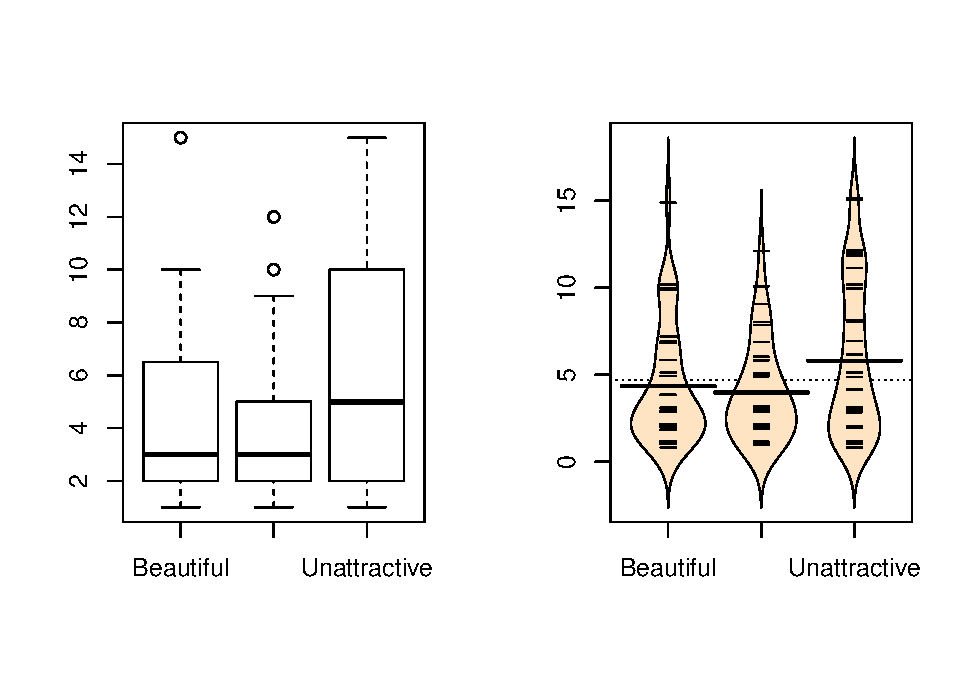
\includegraphics{03-oneWayAnova_files/figure-latex/Figure3-1-1.pdf}
\caption{\label{fig:Figure3-1}Boxplot and beanplot of the sentences (years) for the three
treatment groups.}
\end{figure}

\begin{Shaded}
\begin{Highlighting}[]
\KeywordTok{favstats}\NormalTok{(Years}\OperatorTok{~}\NormalTok{Attr,}\DataTypeTok{data=}\NormalTok{MockJury)}
\end{Highlighting}
\end{Shaded}

\begin{verbatim}
##           Attr min Q1 median   Q3 max     mean       sd  n missing
## 1    Beautiful   1  2      3  6.5  15 4.333333 3.405362 39       0
## 2      Average   1  2      3  5.0  12 3.973684 2.823519 38       0
## 3 Unattractive   1  2      5 10.0  15 5.810811 4.364235 37       0
\end{verbatim}

There are slight differences in the sample sizes in the three groups
with 37 \emph{Unattractive}, 38 \emph{Average} and 39 \emph{Beautiful}
group responses, providing a data set has a total sample size of
\(N=114\). The \emph{Beautiful} and \emph{Average} groups do not appear
to be very different with means of 4.33 and 3.97 years. In Chapter
\ref{chapter2}, we found moderate evidence regarding the difference in
\emph{Average}and \emph{Unattractive}. It is less clear whether we might
find evidence of a difference between \emph{Beautiful} and
\emph{Unattractive} groups since we are comparing means of 5.81 and 4.33
years. All the distributions appear to be right skewed with relatively
similar shapes. The variability in \emph{Average} and
\emph{Unattractive} groups seems like it could be slightly different
leading to an overall concern of whether the variability is the same in
all the groups.

\section{Linear model for One-Way ANOVA (cell-means and
reference-coding)}\label{section3-2}

We introduced the statistical model \(y_{ij} = \mu_j+\varepsilon_j\) in
Chapter \ref{chapter2} for the situation with \(j = 1 \text{ or } 2\) to
denote a situation where there were two groups and, for the model that
is consistent with the alternative hypothesis, the means differed. Now
we have three groups and the previous model can be extended to this new
situation by allowing \(j\) to be 1, 2, or 3. Now that we have more than
two groups, we need to admit that what we were doing in Chapter
\ref{chapter2} was actually fitting what is called a
\textbf{\emph{linear model}}. The linear model assumes that the
responses follow a normal distribution with the linear model defining
the mean, all observations have the same variance, and the parameters
for the mean in the model enter linearly. This last condition is hard to
explain at this level of material -- it is sufficient to know that there
models where the parameters enter the model nonlinearly and that they
are beyond the scope of this course. The result of this constraint is
that we will be able to use the same general modeling framework for the
methods introduced in Chapters \ref{chapter3}, \ref{chapter4},
\ref{chapter6}, \ref{chapter7}, and \ref{chapter8}.

As in Chapter \ref{chapter2}, we have a null hypothesis that defines a
situation (and model) where all the groups have the same mean.
Specifically, the \textbf{\emph{null hypothesis}} in the general
situation with \(J\) groups (\(J\ge 2\)) is to have all the
\textbf{true} group means equal,

\[H_0:\mu_1 = \ldots \mu_J.\]

This defines a model where all the groups have the same mean so it can
be defined in terms of a single mean, \(\mu\), for the \(i^{th}\)
observation from the \(j^{th}\) group as
\(y_{ij} = \mu+\varepsilon_{ij}\). This is not the model that most
researchers want to be the final description of their study as it
implies no difference in the groups. There is more caution required to
specify the alternative hypothesis with more than two groups. The
\textbf{\emph{alternative hypothesis}} needs to be the logical negation
of this null hypothesis of all groups having equal means; to make the
null hypothesis false, we only need one group to differ but more than
one group could differ from the others. Essentially, there are many ways
to ``violate'' the null hypothesis so we choose some delicate wording
for the alternative hypothesis when there are more than 2 groups.
Specifically, we state the alternative as

\[H_A: \text{ Not all } \mu_j \text{ are equal}\]

or, in words, \textbf{at least one of the true means differs among the J
groups}. You will be attracted to trying to say that all means are
different in the alternative but we do not put this strict a requirement
in place to reject the null hypothesis. The alternative model allows all
the true group means to differ but does require that they differ with

\[{\color{red}{\mu_j}}+\varepsilon_{ij}.\]

This linear model states that the response for the \(i^{th}\)
observation in the \(j^{th}\) group, \(\mathbf{y_{ij}}\), is modeled
with a group \(j\) (\(j=1, \ldots, J\)) population mean, \(\mu_j\), and
a random error for each subject in each group \(\varepsilon_{ij}\), that
we assume follows a normal distribution and that all the random errors
have the same variance, \(\sigma^2\). We can write the assumption about
the random errors, often called the \textbf{\emph{normality
assumption}}, as \(\varepsilon_{ij} \sim N(0,\sigma^2)\). There is a
second way to write out this model that allows extension to more complex
models discussed below, so we need a name for this version of the model.
The model written in terms of the \({\color{red}{\mu_j}}\text{'s}\) is
called the \textcolor{red}{\textbf{cell means model}} and is the easier
version of this model to understand.

One of the reasons we learned about beanplots is that it helps us
visually consider all the aspects of this model. In the right panel of
Figure \ref{fig:Figure3-1}, we can see the wider, bold horizontal lines
that provide the estimated group means. The bigger the differences in
the sample means, the more likely we are to find evidence against the
null hypothesis. You can also see the null model on the plot that
assumes all the groups have the same as displayed in the dashed
horizontal line at 4.7 years (the R code below shows the overall mean of
\emph{Years} is 4.7). While the hypotheses focus on the means, the model
also contains assumptions about the distribution of the responses --
specifically that the distributions are normal and that all the groups
have the same variability. As discussed previously, it appears that the
distributions are right skewed and the variability might not be the same
for all the groups. The boxplot provides the information about the skew
and variability but since it doesn't display the means it is not
directly related to the linear model and hypotheses we are considering.

\begin{Shaded}
\begin{Highlighting}[]
\KeywordTok{mean}\NormalTok{(MockJury}\OperatorTok{$}\NormalTok{Years)}
\end{Highlighting}
\end{Shaded}

\begin{verbatim}
## [1] 4.692982
\end{verbatim}

There is a second way to write out the One-Way ANOVA model that provides
a framework for extensions to more complex models described in Chapter
\ref{chapter4} and beyond. The other \textbf{\emph{parameterization}}
(way of writing out or defining) of the model is called the
\textcolor{purple}{\textbf{reference-coded model}} since it writes out
the model in terms of a\\
\textbf{\emph{baseline group}} and deviations from that baseline or
reference level. The reference-coded model for the \(i^{th}\) subject in
the \(j^{th}\) group is
\(y_{ij} =\color{purple}{\boldsymbol{\alpha + \tau_j}}+\varepsilon_{ij}\)
where \(\color{purple}{\boldsymbol{\alpha}}\) (alpha) is the true mean
for the baseline group (first alphabetically) and the
\(\color{purple}{\boldsymbol{\tau_j}}\) (tau \(j\)) are the deviations
from the baseline group for group \(j\). The deviation for the baseline
group, \(\color{purple}{\boldsymbol{\tau_1}}\), is always set to 0 so
there are really just deviations for groups 2 through \(J\). The
equivalence between the two models can be seen by considering the mean
for the first, second, and \(J^{th}\) groups in both models:

\begin{tabular}{l|l|l}
\hline
 & Cell means: & Reference-coded:\\
\hline
Group 1: & \$\{\textbackslash{}color\{red\}\{\textbackslash{}mu\_1\}\}\$ & \$\{\textbackslash{}color\{purple\}\{\textbackslash{}boldsymbol\{\textbackslash{}alpha\}\}\}\$\\
\hline
Group 2: & \$\{\textbackslash{}color\{red\}\{\textbackslash{}mu\_2\}\}\$ & \$\{\textbackslash{}color\{red\}\{\textbackslash{}boldsymbol\{\textbackslash{}tau\_2\}\}\}\$\\
\hline
\$\textbackslash{}ldots\$ & \$\textbackslash{}ldots\$ & \$\textbackslash{}ldots\$\\
\hline
Group \$J\$: & \$\{\textbackslash{}color\{red\}\{\textbackslash{}mu\_J\}\}\$ & \$\{\textbackslash{}color\{purple\}\{\textbackslash{}boldsymbol\{\textbackslash{}tau\_J\}\}\}\$\\
\hline
\end{tabular}

The hypotheses for the reference-coded model are similar to those in the
cell-means coding except that they are defined in terms of the
deviations, \({\color{purple}{\boldsymbol{\tau_j}}}\). The null
hypothesis is that there is no deviation from the baseline for any group
-- that all the \({\color{purple}{\boldsymbol{\tau_j\text{'s}}}}=0\),

\[\boldsymbol{H_0: \tau_2=\ldots=\tau_J=0}.\]

The alternative hypothesis is that at least one of the deviations is not
0,

\[\boldsymbol{H_A:} \textbf{ Not all } \boldsymbol{\tau_j} \textbf{ equal } \bf{0}.\]

In this chapter, you are welcome to use either version (unless we
instruct you otherwise) but we have to use the reference-coding in
subsequent chapters. The next task is to learn how to use R's linear
model \texttt{lm} function to get estimates of the parameters in each
model, but first a quick review of these new ideas:

\textcolor{red}{\textbf{Cell Means Version}}

\begin{itemize}
\item
  \(H_0: {\color{red}{\mu_1=\ldots\mu_J}}\) ~~~~~~~ ~~~
  \(H_A: {\color{red}{\text{ Not all } \mu_j \text{ equal}}}\)
\item
  Null hypothesis in words: No difference in the true means between the
  groups.
\item
  Null model \(y_{ij} = \mu_j+\varepsilon_{ij}\)
\item
  Alternative hypothesis in words: At least one of the true means
  differs between the groups.
\item
  Alternative model: \(y_{ij} = \color{red}{\mu_j}+\varepsilon_{ij}.\)
\end{itemize}

\textcolor{purple}{\textbf{Reference-coded Version}}

\begin{itemize}
\item
  \(H_0: \color{purple}{\boldsymbol{\tau_2 \ldots \tau_J = 0}}\)
  ~~~~~~~~
  \(H_A: \color{purple}{\text{ Not all } \tau_j \text{ equal}}\)
\item
  Null hypothesis in words: No deviation of the true mean for any groups
  from the baseline group.
\item
  Null model: \(y_{ij} =\boldsymbol{\alpha} + \tau_j+\varepsilon_{ij}\)
\item
  Alternative hypothesis in words: At least one of the true deviations
  is different from 0 or that at least one group has a different true
  mean than the baseline group.
\item
  Alternative model:
  \(y_{ij} =\color{purple}{\boldsymbol{\alpha + \tau_j}}+\varepsilon_{ij}\)
\end{itemize}

In order to estimate the models discussed above, the \texttt{lm}
function is used. If you look closely in the code for the rest of the
book, any model for a quantitative response will use this function,
suggesting a common thread in the most commonly used statistical models.
The \texttt{lm} function continues to use the same format as previous
functions, \texttt{lm(Y\textasciitilde{}X,\ data=datasetname)}. It ends
up that this code will give you the reference-coded version of the model
by default (R thinks it is that important!). We want to start with the
cell-means version of the model, so we have to override the standard
technique and add a ``\texttt{-1}'' to the formula interface to tell R
that we want to the cell-means coding. Generally, this looks like
\texttt{lm(Y\textasciitilde{}X-1\ ,\ data=datasetname).} Once we fit a
model in R, the \texttt{summary} function run on the model provides a
useful ``summary'' of the model coefficients and a suite of other
potentially interesting information. When fitting this version of the
One-Way ANOVA model, you will find a row of output for each group
relating the \(\mu_j\text{'s}\). The output contains columns for an
estimate (\texttt{Estimate}), standard error (\texttt{Std.Error}),
\(t\)-value (\texttt{t\ value}), and p-value
(\texttt{Pr(\textgreater{}\textbar{}t\textbar{})}). We'll learn to use
all the output in the following material, but for now just focus on the
estimates of the parameters that the function provides that we put in
bold.

\begin{Shaded}
\begin{Highlighting}[]
\NormalTok{lm1 <-}\StringTok{ }\KeywordTok{lm}\NormalTok{(Years }\OperatorTok{~}\StringTok{ }\NormalTok{Attr}\OperatorTok{-}\DecValTok{1}\NormalTok{, }\DataTypeTok{data=}\NormalTok{MockJury)}
\KeywordTok{summary}\NormalTok{(lm1)}
\end{Highlighting}
\end{Shaded}

\begin{verbatim}
## 
## Call:
## lm(formula = Years ~ Attr - 1, data = MockJury)
## 
## Residuals:
##     Min      1Q  Median      3Q     Max 
## -4.8108 -2.8108 -0.9737  2.1892 10.6667 
## 
## Coefficients:
##                  Estimate Std. Error t value Pr(>|t|)
## AttrBeautiful      4.3333     0.5730   7.563 1.23e-11
## AttrAverage        3.9737     0.5805   6.845 4.41e-10
## AttrUnattractive   5.8108     0.5883   9.878  < 2e-16
## 
## Residual standard error: 3.578 on 111 degrees of freedom
## Multiple R-squared:  0.6449, Adjusted R-squared:  0.6353 
## F-statistic: 67.21 on 3 and 111 DF,  p-value: < 2.2e-16
\end{verbatim}

\begin{longtable}[]{@{}ccccc@{}}
\toprule
\begin{minipage}[b]{0.27\columnwidth}\centering\strut
~\strut
\end{minipage} & \begin{minipage}[b]{0.13\columnwidth}\centering\strut
Estimate\strut
\end{minipage} & \begin{minipage}[b]{0.16\columnwidth}\centering\strut
Std. Error\strut
\end{minipage} & \begin{minipage}[b]{0.12\columnwidth}\centering\strut
t value\strut
\end{minipage} & \begin{minipage}[b]{0.12\columnwidth}\centering\strut
Pr(\textgreater{}\textbar{}t\textbar{})\strut
\end{minipage}\tabularnewline
\midrule
\endhead
\begin{minipage}[t]{0.27\columnwidth}\centering\strut
\textbf{AttrBeautiful}\strut
\end{minipage} & \begin{minipage}[t]{0.13\columnwidth}\centering\strut
\textbf{4.33}\strut
\end{minipage} & \begin{minipage}[t]{0.16\columnwidth}\centering\strut
0.573\strut
\end{minipage} & \begin{minipage}[t]{0.12\columnwidth}\centering\strut
7.56\strut
\end{minipage} & \begin{minipage}[t]{0.12\columnwidth}\centering\strut
1.23e-11\strut
\end{minipage}\tabularnewline
\begin{minipage}[t]{0.27\columnwidth}\centering\strut
\textbf{AttrAverage}\strut
\end{minipage} & \begin{minipage}[t]{0.13\columnwidth}\centering\strut
\textbf{3.97}\strut
\end{minipage} & \begin{minipage}[t]{0.16\columnwidth}\centering\strut
0.58\strut
\end{minipage} & \begin{minipage}[t]{0.12\columnwidth}\centering\strut
6.85\strut
\end{minipage} & \begin{minipage}[t]{0.12\columnwidth}\centering\strut
4.41e-10\strut
\end{minipage}\tabularnewline
\begin{minipage}[t]{0.27\columnwidth}\centering\strut
\textbf{AttrUnattractive}\strut
\end{minipage} & \begin{minipage}[t]{0.13\columnwidth}\centering\strut
\textbf{5.81}\strut
\end{minipage} & \begin{minipage}[t]{0.16\columnwidth}\centering\strut
0.588\strut
\end{minipage} & \begin{minipage}[t]{0.12\columnwidth}\centering\strut
9.88\strut
\end{minipage} & \begin{minipage}[t]{0.12\columnwidth}\centering\strut
6.86e-17\strut
\end{minipage}\tabularnewline
\bottomrule
\end{longtable}

In general, we denote estimated parameters with a hat over the parameter
of interest to show that it is an estimate. For the true mean of group
\(j\), \(\mu_j\), we estimate it with \(\hat{\mu}_j\), which is just the
sample mean for group \(j\), \(\bar{x}_j\). The model suggests an
estimate for each observation that we denote as \(\hat{y}_{ij}\) that we
will also call a \textbf{\emph{fitted value}} based on the model being
considered. The three estimates are bolded in the previous output, with
the same estimate used for all observations in the same group. R tries
to help you to sort out which row of output corresponds to which group
by appending the group name l with the variable name. Here, the variable
name was \texttt{Attr} and the first group alphabetically was
\emph{Beautiful}, so R provides a row labeled \texttt{AttrBeautiful}
with an estimate of 4.3333. The sample means from the three groups can
be seen to directly match that and the other two results.

\begin{Shaded}
\begin{Highlighting}[]
\KeywordTok{mean}\NormalTok{(Years }\OperatorTok{~}\StringTok{ }\NormalTok{Attr, }\DataTypeTok{data=}\NormalTok{MockJury)}
\end{Highlighting}
\end{Shaded}

\begin{verbatim}
##    Beautiful      Average Unattractive 
##     4.333333     3.973684     5.810811
\end{verbatim}

The reference-coded version of the same model is more complicated but
ends up giving the same results once we understand what it is doing. It
uses a different parameterization to accomplish this so has different
model output. Here is the model summary:

\begin{Shaded}
\begin{Highlighting}[]
\NormalTok{lm2 <-}\StringTok{ }\KeywordTok{lm}\NormalTok{(Years }\OperatorTok{~}\StringTok{ }\NormalTok{Attr, }\DataTypeTok{data=}\NormalTok{MockJury)}
\KeywordTok{summary}\NormalTok{(lm2)}
\end{Highlighting}
\end{Shaded}

\begin{verbatim}
## 
## Call:
## lm(formula = Years ~ Attr, data = MockJury)
## 
## Residuals:
##     Min      1Q  Median      3Q     Max 
## -4.8108 -2.8108 -0.9737  2.1892 10.6667 
## 
## Coefficients:
##                  Estimate Std. Error t value Pr(>|t|)
## (Intercept)        4.3333     0.5730   7.563 1.23e-11
## AttrAverage       -0.3596     0.8157  -0.441   0.6601
## AttrUnattractive   1.4775     0.8212   1.799   0.0747
## 
## Residual standard error: 3.578 on 111 degrees of freedom
## Multiple R-squared:  0.04754,    Adjusted R-squared:  0.03038 
## F-statistic:  2.77 on 2 and 111 DF,  p-value: 0.067
\end{verbatim}

The estimated model coefficients are \(\hat{\alpha} = 4.333\) years,
\(\hat{tau}_2 =-0.3596\) years, \(\hat{\tau}_3=1.4775\) years where R
selected group 1 for \emph{Beautiful}, 2 for \emph{Average}, and 3 for
\emph{Unattractive}. The way you can figure out the baseline group
(group 1 is \emph{Beautiful} here) is to see which category label is
\emph{not present} in the output. \textbf{The baseline level is
typically the first group label alphabetically}, but you should always
check this. Based on these definitions, there are interpretations
available for each coefficient. For \(\hat{\alpha} = 4.333\) years, this
is an estimate of the mean sentencing time for the
\emph{Beautiful}group. \(\hat{\tau}_2 =-0.3596\) years is the deviation
of the \emph{Average} group's mean from the \emph{Beautiful} groups mean
(specifically, it is \(0.36\) years lower). Finally,
\(\hat{\tau}_3=1.4775\) years tells us that the \emph{Unattractive}
group mean sentencing time is 1.48 years higher than time. These
interpretations lead directly to reconstructing the estimated means for
each group by combining the baseline and pertinent deviations as shown
in Table \ref{tab:Table3-1}.




\begin{table}

\caption{\label{tab:Table3-1}Constructing group mean estimates from the reference-coded
linear model estimates.}
\centering
\begin{tabular}[t]{l|l|l}
\hline
Group & Formula & Estimates\\
\hline
Beautiful & \$\textbackslash{}hat\{\textbackslash{}alpha\}\$ & **4.3333** years\\
\hline
Average & \$\textbackslash{}hat\{\textbackslash{}alpha\}+\textbackslash{}hat\{\textbackslash{}tau\}\_2\$ & 4.3333 - 0.3596 = **3.974** years\\
\hline
Unattractive & \$\textbackslash{}hat\{\textbackslash{}alpha\}+\textbackslash{}hat\{\textbackslash{}tau\}\_3\$ & 4.3333 + 1.4775 = **5.811** years\\
\hline
\end{tabular}
\end{table}

We can also visualize the results of our linear models using what are
called \textbf{\emph{term-plots}} or \textbf{\emph{effect-plots}} (from
the \texttt{effects} package; \citet{Fox2003}, \citep{R-effects}) as
displayed in Figure \ref{fig:Figure3-2}. We don't want to use the word
``effect'' for these model components unless we have random assignment
in the study design so we generically call these
\textbf{\emph{term-plots}} as they display terms or components from the
model in hopefully useful ways to aid in model interpretation even in
the presence of complicated model parameterizations. Specifically, these
plots take an estimated model and show you its estimates along with 95\%
confidence intervals generated by the linear model. To make this plot,
you need to install and load the \texttt{effects} package and then use
\texttt{plot(allEffects(...))} functions together on the \texttt{lm}
object called \texttt{lm2} that was estimated above. You can find the
correspondence between the displayed means and the estimates that were
constructed in Table \ref{tab:Table3-1}.




\begin{Shaded}
\begin{Highlighting}[]
\KeywordTok{require}\NormalTok{(effects)}
\KeywordTok{plot}\NormalTok{(}\KeywordTok{allEffects}\NormalTok{(lm2))}
\end{Highlighting}
\end{Shaded}

\begin{figure}
\centering
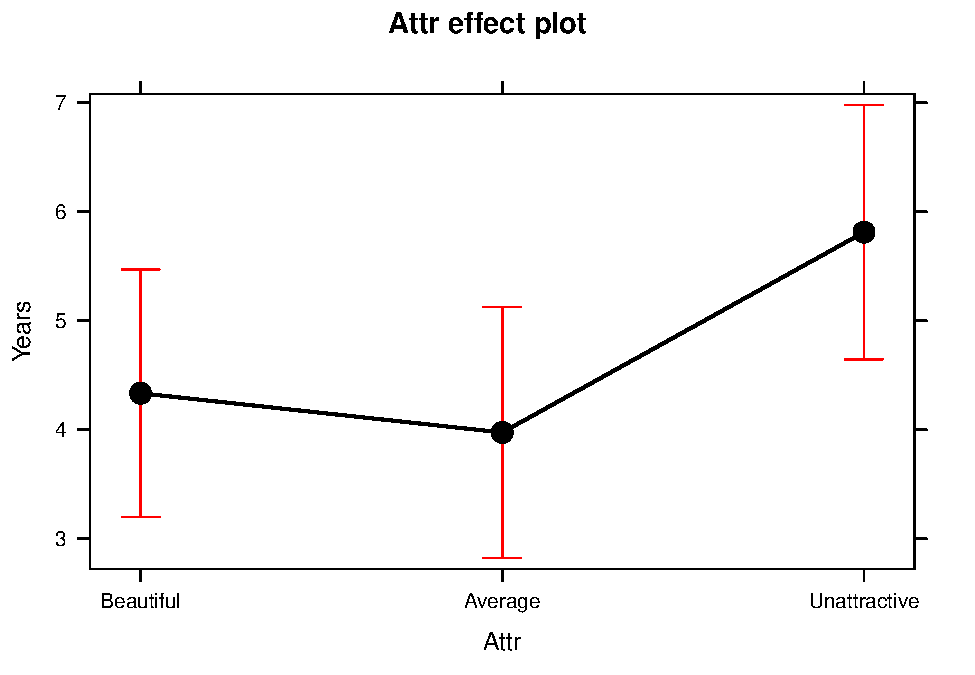
\includegraphics{03-oneWayAnova_files/figure-latex/Figure3-2-1.pdf}
\caption{\label{fig:Figure3-2}Plot of the estimated group mean sentences from the
reference-coded model for the MockJury data.}
\end{figure}

In order to assess evidence for having different means for the groups,
we will compare either of the previous models (cell-means or
reference-coded) to a null model based on the null hypothesis
(\(H_0: \mu_1 = \ldots = \mu_J\)) which implies a model of
\(\color{red}{y_{ij} = \mu_j}+\varepsilon_{ij}\) in the cell-means
version where \({\color{red}{\mu}}\) is a common mean for all the
observations. We will call this the \textcolor{red}{\textbf{mean-only}}
model since it only has a single mean in it. In the reference-coding
version of the model, we have a null hypothesis that
\(H_0: \tau_2 = \ldots = \tau_J = 0\), so the ``mean-only'' model is
\(\color{purple}{y_{ij} =\boldsymbol{\alpha}+\varepsilon_{ij}}\) with
\(\color{purple}{\boldsymbol{\alpha}}\) having the same definition as
\(\color{red}{\mu}\) for the cell means model -- it forces a common
value for the mean for all the groups. Moving from the
\emph{reference-coded} model to the \emph{mean-only} model is also an
example of a situation where we move from a ``full'' model to a
``reduced'' model by setting some coefficients in the ``full'' model to
0 and, by doing this, get a simpler or ``reduced'' model. Simple models
can be good as they are easier to groups that suggests no difference in
the groups is not a very exciting result in most, but not all,
situations\footnote{Suppose we were doing environmental monitoring and
  were studying asbestos levels in soils. We might be hoping that the
  mean-only model were reasonable to use if the groups being compared
  were in remediated areas and in areas known to have never been
  contaminated.}. In order for R to provide results for the mean-only
model, we remove the grouping variable, \texttt{Attr}, from the model
formula and just include a ``1''. The \texttt{(Intercept)} row of the
output provides the estimate for the mean-only model as a reduced model
from either the cell-means or reference-coded models when we assume that
the mean is the same for all groups:

\begin{Shaded}
\begin{Highlighting}[]
\NormalTok{lm3 <-}\StringTok{ }\KeywordTok{lm}\NormalTok{(Years }\OperatorTok{~}\StringTok{ }\DecValTok{1}\NormalTok{, }\DataTypeTok{data=}\NormalTok{MockJury)}
\KeywordTok{summary}\NormalTok{(lm3)}
\end{Highlighting}
\end{Shaded}

\begin{verbatim}
## $coefficients
##             Estimate Std. Error  t value     Pr(>|t|)
## (Intercept) 4.692982  0.3403532 13.78857 5.765681e-26
\end{verbatim}

This model provides an estimate of the common mean for all observations
of \(4.693 = \hat{\mu} = \hat{\alpha}\) years. This value also is the
dashed, horizontal line in the beanplot in Figure \ref{fig:Figure3-1}.
Some people call this mean-only estimate the grand or overall mean.

\section{One-Way ANOVA Sums of Squares, Mean Squares, and
F-test}\label{section3-3}

The previous discussion showed two ways of parameterizing models for the
One-Way ANOVA model and getting estimates from output but still hasn't
addressed how to assess evidence related to whether the observed
differences in the means among the groups is ``real''. In this section,
we develop what is called the \textbf{\emph{ANOVA F-test}} that provides
a method of aggregating the differences among the means of 2 or more
groups and testing our null hypothesis of no difference in the means vs
the alternative. In order to develop the test, some additional notation
is needed. The sample size in each group is denoted \(n_j\) and the
total sample size is
\(\boldsymbol{N=\Sigma n_j = n_1 + n_2 + \ldots + n_J}\) where
\(\Sigma\) (capital sigma) means ``add up over whatever follows''. An
estimated \textbf{\emph{residual}} (\(e_{ij}\)) is the difference
between an observation, \(y_{ij}\), and the model estimate,
\(\hat{y}_{ij} = \hat{\mu}_j\), for that observation,
\(y_{ij}-\hat{y}_{ij} = e_{ij}\). It is basically what is left over that
the mean part of the model (\(\hat{\mu}_{j}\)) does not explain. It is
also a window into how ``good'' the model might be.

Consider the four different fake results for a situation with four
groups (\(J=4\)) displayed in Figure \ref{fig:Figure3-3}. Which of the
different results shows the most and least evidence of differences in
the means? In trying to answer this, think about both how different the
means are (obviously important) and how variable the results are around
the mean. These situations were created to have the same means in
Scenarios 1 and 2 as well as matching means in Scenarios 3 and 4. The
variability around the means matches by shading (lighter or darker). In
Scenarios 1 and 2, the differences in the means is smaller than in the
other two results. But Scenario 2 should provide more evidence of what
little difference in present than Scenario 1 because it has less
variability around the means. The best situation for finding group
differences here is Scenario 4 since it has the largest difference in
the means and the least variability around those means. Our test
statistic somehow needs to allow a comparison of the variability in the
means to the overall variability to help us get results that reflect
that Scenario 4 has the strongest evidence of a difference and Scenario
1 would have the least.





\begin{figure}
\centering
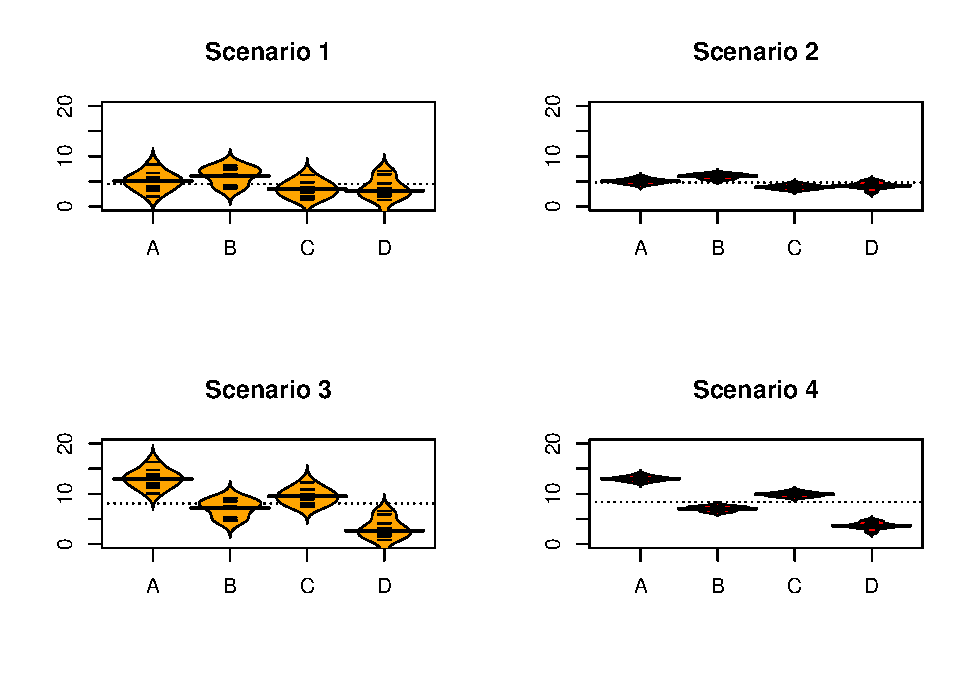
\includegraphics{03-oneWayAnova_files/figure-latex/Figure3-3-1.pdf}
\caption{\label{fig:Figure3-3}Demonstration of different amounts of difference in means
relative to variability. Scenarios have same means in rows and same
variance around means in columns of plot.}
\end{figure}

The statistic that allows the comparison of relative amounts of
variation is called the \textbf{\emph{ANOVA F-statistic}} . It is
developed using \textbf{\emph{sums of squares}} which are measures of
total variation like are used in the numerator of the standard deviation
(\(\Sigma_1^N(y_i-\bar{y})^2\)) that took all the observations,
subtracted the mean, squared the differences, and then added up the
results over all the observations to generate a measure of total
variability. With multiple groups, we will focus on decomposing that
total variability (\textbf{\emph{Total Sums of Squares}}) into
variability among the means (we'll call this \textbf{\emph{Explanatory
Variable}} \(\mathbf{A}\textbf{'s}\) \textbf{\emph{Sums of Squares}})
and variability in the residuals or errors ( \textbf{\emph{Error Sums of
Squares}}). We define each of these quantities in the One-Way ANOVA
situation as follows:

\begin{itemize}
\item
  \(\textbf{SS}_{\textbf{Total}} =\) Total Sums of Squares
  \(= \Sigma^J_{j=1}\Sigma^{n_j}_{i=1}(y_{ij}-\bar{\bar{y}})^2\)

  \begin{itemize}
  \item
    This is the total variation in the responses around the overall or
    \textbf{\emph{grand mean}} (\(\bar{\bar{y}}\), the estimated mean
    for all the observations and available from the mean-only model).
  \item
    By summing over all \(n_j\) observations in each group,
    \(\Sigma^{n_j}_{i=1}(\ )\), and then adding those results up across
    the groups, \(\Sigma^J_{j=1}(\ )\), we accumulate the variation
    across all \(N\) observations.
  \item
    Note: this is the residual variation if the null model is used, so
    there is no further decomposition possible for that model.
  \item
    This is also equivalent to the numerator of the sample variance,
    \(\Sigma^{N}_{1}(y_{i}-\bar{y})^2\) which is what you get when you
    ignore the information on the potential differences in the groups.
  \end{itemize}
\item
  \(\textbf{SS}_{\textbf{A}} =\) Explanatory Variable \emph{A}'s Sums of
  Squares
  \(=\Sigma^J_{j=1}\Sigma^{n_j}_{i=1}(\bar{y}_{i}-\bar{\bar{y}})^2 =\Sigma^J_{j=1}n_j(\bar{y}_{i}-\bar{\bar{y}})^2\)

  \begin{itemize}
  \item
    This is the variation in the group means around the grand mean based
    on the explanatory variable \(A\).
  \item
    Also called sums of squares for the treatment, regression, or model.
  \end{itemize}
\item
  \(\textbf{SS}_E =\) Error (Residual) Sums of Squares
  \(=\Sigma^J_{j=1}\Sigma^{n_j}_{i=1}(y_{ij}-\bar{y})^2 =\Sigma^J_{j=1}\Sigma^{n_j}_{i=1}(e_{ij})^2\)

  \begin{itemize}
  \item
    This is the variation in the responses around the group means.
  \item
    Also called the sums of squares for the residuals, with the second
    version of the formula showing that it is just the squared residuals
    added up across all the observations.
  \end{itemize}
\end{itemize}

The possibly surprising result given the mass of notation just presented
is that the total sums of squares is \textbf{ALWAYS} equal to the sum of
explanatory variable \(A\text{'s}\) sum of squares and the error sums of
squares,

\[\textbf{SS}_{\textbf{Total}} \mathbf{=} \textbf{SS}_\textbf{A} \mathbf{+} \textbf{SS}_\textbf{E}.\]

This equality means that if the \(\textbf{SS}_\textbf{A}\) goes up, then
the \(\textbf{SS}_\textbf{E}\) must go down if
\(\textbf{SS}_{\textbf{Total}}\) remains the same. This result is called
the \textbf{\emph{sums of squares decomposition formula}}. We use these
results to build our test statistic and organize this information in
what is called an \textbf{\emph{ANOVA table}}. The ANOVA table is
generated using the \texttt{anova} function applied to the
reference-coded model, \texttt{lm2} :

\begin{Shaded}
\begin{Highlighting}[]
\NormalTok{lm2<-}\KeywordTok{lm}\NormalTok{(Years }\OperatorTok{~}\StringTok{ }\NormalTok{Attr, }\DataTypeTok{data=}\NormalTok{MockJury)}
\KeywordTok{anova}\NormalTok{(lm2)}
\end{Highlighting}
\end{Shaded}

\begin{verbatim}
## Analysis of Variance Table
## 
## Response: Years
##            Df  Sum Sq Mean Sq F value Pr(>F)
## Attr        2   70.94  35.469    2.77  0.067
## Residuals 111 1421.32  12.805
\end{verbatim}

Note that the ANOVA table has a row labelled \texttt{Attr}, which
contains information for the grouping variable (we'll generally refer to
this as explanatory variable \(A\) but here it is the picture group that
was randomly assigned), and a row labelled \texttt{Residuals}, which is
synonymous with ``Error''. The Sums of Squares (SS) are available in the
\texttt{Sum\ Sq} column. It doesn't show a row for ``Total'' but the
\(\textbf{SS}_{\textbf{Total}} \mathbf{=} \textbf{SS}_\textbf{A} \mathbf{+} \textbf{SS}_\textbf{E} = 1492.26\).

\begin{Shaded}
\begin{Highlighting}[]
\FloatTok{70.94} \OperatorTok{+}\StringTok{ }\FloatTok{1421.32}
\end{Highlighting}
\end{Shaded}

\begin{verbatim}
## [1] 1492.26
\end{verbatim}

It may be easiest to understand the \emph{sums of squares decomposition}
by connecting it to our permutation ideas. In a permutation situation,
the total variation (\(SS_{Total}\)) cannot change -- it is the same
responses varying around the grand mean. However, the amount of
variation attributed to variation among the means and in the residuals
can change if we change which observations go with which group. In
Figure \ref{fig:Figure3-4} (panel a), the means, sums of squares, and
95\% confidence intervals for each mean are displayed for the three
treatment levels from the original prisoner rating data. Three permuted
versions of the data set are summarized in panels (b), (c), and (d). The
\(\text{SS}_A\) is 70.9 in the real data set and between 6.6 and 11 in
the permuted data sets. If you had to pick among the plots for the one
with the most evidence of a difference in the means, you hopefully would
pick panel (a). This visual ``unusualness'' suggests that this observed
result is unusual relative to the possibilities under permutations,
which are, again, the possibilities tied to having the null hypothesis
being true. But note that the differences here are not that great
between these three permuted data sets and the real one. It is likely
that at least some of you might have selected panel (d) as also looking
like it shows some evidence of differences (maybe not the most?) as it
also looks like it shows some evidence differences.

One way to think about \(\textbf{SS}_\textbf{A}\) is that it is a
function that converts the variation in the group means into a single
value. This makes it a reasonable test statistic in a permutation
testing context. By comparing the observed \(\text{SS}_A =\) 70.9 to the
permutation results of 6.5, 9.7, and 40.5 we see that the observed
result is much more extreme than the three alternate versions. In
contrast to our previous test statistics where positive and negative
differences were possible, \(\text{SS}_A\) is always positive with a
value of 0 corresponding to no variation in the means. The larger the
\(\text{SS}_A\), the more variation there is in the means. The
permutation p-value for the alternative hypothesis of \textbf{some} (not
of greater or less than!) difference in the true means of the groups
will involve counting the number of permuted \(SS_A^*\) results that are
larger than what we observed.








\begin{verbatim}
## [1] 70.93836
\end{verbatim}

\begin{figure}
\centering
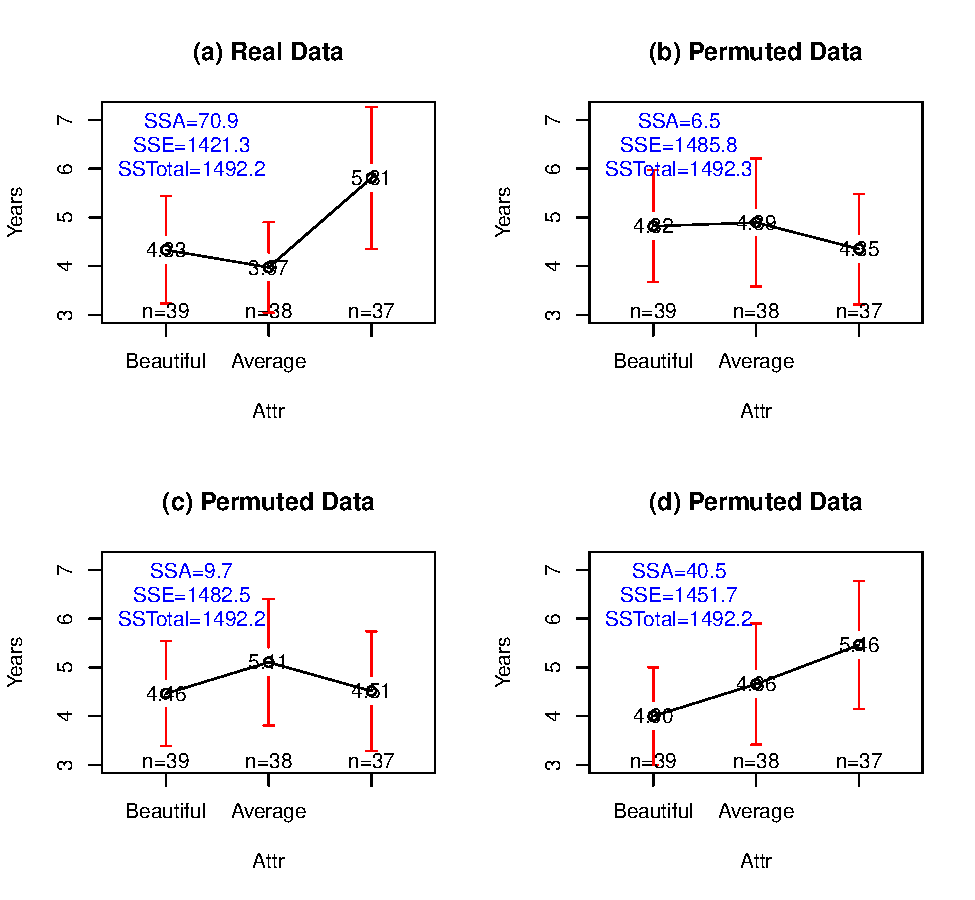
\includegraphics{03-oneWayAnova_files/figure-latex/Figure3-4-1.pdf}
\caption{\label{fig:Figure3-4}Plot of means and 95\% confidence intervals for the three
groups for the real data (a) and three different permutations of the
treatment labels to the same responses in (b), (c), and (d). Note that
SSTotal is always the same but the different amounts of variation
associated with the means (SSA) or the errors (SSE) changes in
permutation.}
\end{figure}

To do a permutation test, we need to be able to calculate and extract
the \(\text{SS}_A\) value. In the ANOVA table, it is in the first row
and is the second number and we can use the bracket, \texttt{{[},\ {]}},
referencing to extract that number from the ANOVA table that
\texttt{anova} produces with
\texttt{anova(lm(Years\textasciitilde{}Attr,\ data=MockJury)){[}1,\ 2{]}}.
We'll store the observed value of \(\text{SS}_A\) in \texttt{Tobs},
reusing some ideas from Chapter @ref\{chapter2\}.

\begin{Shaded}
\begin{Highlighting}[]
\NormalTok{Tobs <-}\StringTok{ }\KeywordTok{anova}\NormalTok{(}\KeywordTok{lm}\NormalTok{(Years}\OperatorTok{~}\NormalTok{Attr,}\DataTypeTok{data=}\NormalTok{MockJury))[}\DecValTok{1}\NormalTok{,}\DecValTok{2}\NormalTok{]; Tobs}
\end{Highlighting}
\end{Shaded}

\begin{verbatim}
## [1] 70.93836
\end{verbatim}

The following code performs the permutations \texttt{B=1,000} times
using the \texttt{shuffle} function, builds up a vector of results in
\texttt{Tobs}, and then makes a plot of the resulting permutation
distribution:







\begin{Shaded}
\begin{Highlighting}[]
\KeywordTok{par}\NormalTok{(}\DataTypeTok{mfrow=}\KeywordTok{c}\NormalTok{(}\DecValTok{1}\NormalTok{,}\DecValTok{2}\NormalTok{))}
\NormalTok{B<-}\StringTok{ }\DecValTok{1000}
\NormalTok{Tstar<-}\KeywordTok{matrix}\NormalTok{(}\OtherTok{NA}\NormalTok{,}\DataTypeTok{nrow=}\NormalTok{B)}
\ControlFlowTok{for}\NormalTok{ (b }\ControlFlowTok{in}\NormalTok{ (}\DecValTok{1}\OperatorTok{:}\NormalTok{B))\{}
\NormalTok{  Tstar[b]<-}\KeywordTok{anova}\NormalTok{(}\KeywordTok{lm}\NormalTok{(Years}\OperatorTok{~}\KeywordTok{shuffle}\NormalTok{(Attr),}\DataTypeTok{data=}\NormalTok{MockJury))[}\DecValTok{1}\NormalTok{,}\DecValTok{2}\NormalTok{]}
\NormalTok{  \}}
\KeywordTok{hist}\NormalTok{(Tstar,}\DataTypeTok{labels=}\NormalTok{T,}\DataTypeTok{ylim=}\KeywordTok{c}\NormalTok{(}\DecValTok{0}\NormalTok{,}\DecValTok{550}\NormalTok{))}
\KeywordTok{abline}\NormalTok{(}\DataTypeTok{v=}\NormalTok{Tobs,}\DataTypeTok{col=}\StringTok{"red"}\NormalTok{,}\DataTypeTok{lwd=}\DecValTok{3}\NormalTok{)}
\KeywordTok{plot}\NormalTok{(}\KeywordTok{density}\NormalTok{(Tstar),}\DataTypeTok{main=}\StringTok{"Density curve of Tstar"}\NormalTok{)}
\KeywordTok{abline}\NormalTok{(}\DataTypeTok{v=}\NormalTok{Tobs,}\DataTypeTok{col=}\StringTok{"red"}\NormalTok{,}\DataTypeTok{lwd=}\DecValTok{3}\NormalTok{)}
\end{Highlighting}
\end{Shaded}

\begin{figure}
\centering
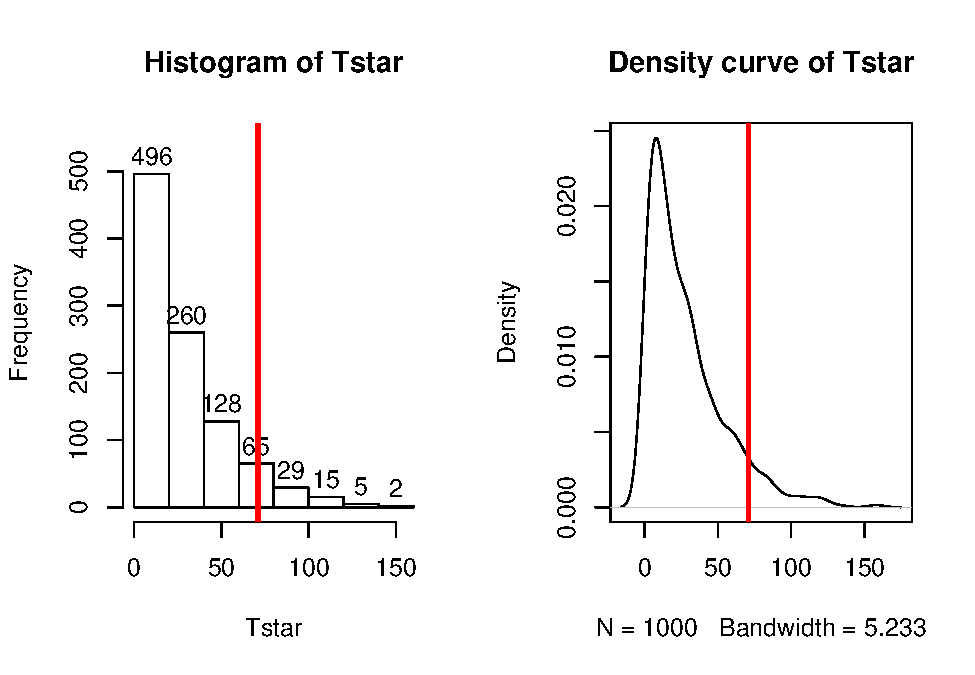
\includegraphics{03-oneWayAnova_files/figure-latex/Figure3-5-1.pdf}
\caption{\label{fig:Figure3-5}Histogram and density curve of permutation distribution of
\(\text{SS}_A\) with the observed value of \(\text{SS}_A\) displayed as
a bold, vertical line. The proportion of results that are larger than
the observed value of \(\text{SS}_A\) provides an estimate of the
p-value.}
\end{figure}

The right-skewed distribution (Figure \ref{fig:Figure3-5}) contains the
distribution of \(\text{SS}_A\text{'s}\) under permutations (where all
the groups are assumed to be equivalent under the null hypothesis).
While the observed result is larger than many of the
\(\text{SS}_A\text{'s}\), there are also many permuted results that are
much larger than observed. The proportion of permuted results that
exceed the observed value is found using \texttt{pdata} as before,
except only for the area to the right of the observed result. We know
that \texttt{Tobs} will always be positive so no absolute values are
required here.

\begin{Shaded}
\begin{Highlighting}[]
\KeywordTok{pdata}\NormalTok{(Tstar,Tobs,}\DataTypeTok{lower.tail=}\NormalTok{F)}
\end{Highlighting}
\end{Shaded}

\begin{verbatim}
## [1] 0.072
\end{verbatim}

This provides a permutation-based p-value of 0.072 and suggests marginal
evidence against the null hypothesis of no difference in the true means.
We would interpret this p-value as saying that there is a 7.2\% chance
of getting a \(\text{SS}_A\) as large or larger than we observed, given
that the null hypothesis is true.

It ends up that some nice parametric statistical results are available
(if our assumptions are met) for the ratio of estimated variances, which
are called \textbf{\emph{Mean Squares}}. To turn sums of squares into
mean square (variance) estimates, we divide the sums of squares by the
amount of free information available. For example, remember the typical
variance estimator introductory statistics,
\(\Sigma^N_1(y_i-\bar{y})^2/(N-1)\)? Your instructor spent some time
trying various approaches to explaining why we have a denominator of
\(N-1\). The most useful for our purposes moving forward is that we
``lose'' one piece of information to estimate the mean and there are
\(N\) deviations around the single mean so we divide by \(N-1\). The
main point is that the sums of squares were divided by something and we
got an estimator for the variance, here of the observations.

Now consider
\(\text{SS}_E = \Sigma^J_{j=1}\Sigma^{n_j}_{i=1}(y_i-\bar{y})^2\) which
still has \(N\) deviations but it varies around the \(J\) means, so the

\[\textbf{Mean Square Error} = \text{MS}_E = \text{SS}_E/(N-J).\]

Basically, we lose \(J\) pieces of information in this calculation
because we have to estimate \(J\) means.

The similar calculation of the \textbf{\emph{Mean Square for variable}}
\(\mathbf{A}\) (\(\text{MS}_A\)) is harder to see in the formula
(\(\text{SS}_A = \Sigma^J_{j=1}n_j(\bar{y}_i-\bar{\bar{y}})^2\)), but
the same reasoning can be used to understand the denominator for forming
\(\text{MS}_A\): there are \(J\) means that vary around the grand mean
so

\[\text{MS}_A = \text{SS}_A/(J-1).\]

In summary, the two mean squares are simply:

\begin{itemize}
\item
  \(\text{MS}_A = \text{SS}_A/(J-1)\), which estimates the variance of
  the group means around the grand mean.
\item
  \(\text{MS}_{\text{Error}} = \text{SS}_{\text{Error}}/(N-J)\), which
  estimates the variation of the errors around the group means.
\end{itemize}

These results are put together using a ratio to define the
\textbf{\emph{ANOVA F-statistic}} (also called the
\textbf{\emph{F-ratio}} ) as

\[F=\text{MS}_A/\text{MS}_{\text{Error}}.\]

If the variability in the means is ``similar'' to the variability in the
residuals, the statistic would have a value around 1. If that
variability is similar then there be no evidence of a difference in the
means. If the \(\text{MS}_A\) is much larger than the \(\text{MS}_E\),
the \(F\)-statistic will provide evidence against the null hypothesis.
The ``size'' of the \(F\)-statistic is formalized by finding the
p-value. The \(F\)-statistic, if assumptions discussed below are met and
we assume the null hypothesis is true, follows what is called an
\(F\)-distribution. The \textbf{\emph{F-distribution}} is a right-skewed
distribution whose shape is defined by what are called the
\textbf{\emph{numerator degrees of freedom}} (\(J-1\)) and the
\textbf{\emph{denominator degrees of freedom}} (\(N-J\)). These names
correspond to the values that we used to calculate the mean squares and
where in the \(F\)-ratio each mean square was used; \(F\)-distributions
are denoted by their degrees of freedom using the convention of \(F\)
(\emph{numerator df}, \emph{denominator df}). Some examples of different
\(F\)-distributions are displayed for you in Figure \ref{fig:Figure3-6}.

The characteristics of the F-distribution can be summarized as:

\begin{itemize}
\item
  Right skewed,
\item
  Nonzero probabilities for values greater than 0,
\item
  Its shape changes depending on the \textbf{numerator} and
  \textbf{denominator DF}, and
\item
  \textbf{Always use the right-tailed area for p-values.}
\end{itemize}






\begin{figure}
\centering
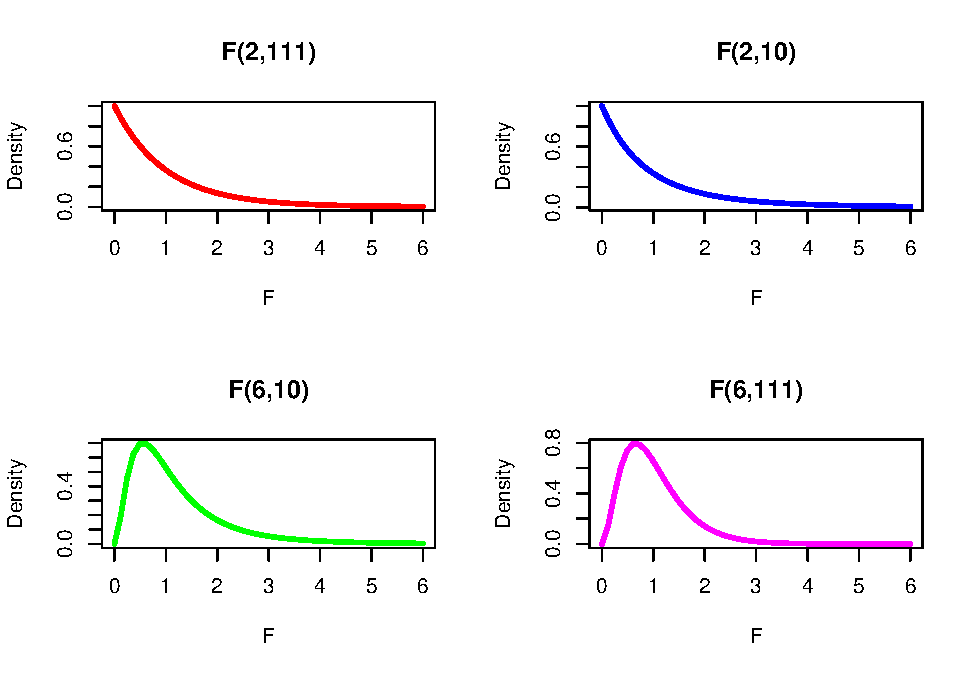
\includegraphics{03-oneWayAnova_files/figure-latex/Figure3-6-1.pdf}
\caption{\label{fig:Figure3-6}Density curves of four different \(F\)-distributions. Upper
left is an \(F(2, 111)\), upper right is \(F(2, 10)\), lower left is
\(F(6, 10)\), and lower right is \(F(6, 111)\). P-values are found using
the areas to the right of the observed \(F\)-statistic value.}
\end{figure}

Now we are ready to discuss an ANOVA table since we know about each of
its components. Note the general format of the ANOVA table is\footnote{Make
  sure you can work from left to right and up and down to fill in the
  ANOVA table given just the necessary information to determine the
  other components -- there is always a question like this on the
  exam\ldots{}}:



\begin{table}

\caption{\label{tab:Table3-2}General One-Way ANOVA table.}
\centering
\begin{tabular}[t]{l|l|l|l|l|l}
\hline
Source & DF & Sums of Squares & Mean Squares & F-ratio & P-value\\
\hline
Variable A & \$J-1\$ & \$\textbackslash{}text\{SS\}\_A\$ & \$\textbackslash{}text\{MS\}\_A=\textbackslash{}text\{SS\}\_A/(J-1)\$ & \$F=\textbackslash{}text\{MS\}\_A/\textbackslash{}text\{MS\}\_E\$ & Right tail of \$F(J-1,N-J)\$\\
\hline
Residuals & \$N-J\$ & \$\textbackslash{}text\{SS\}\_E\$ & \$\textbackslash{}text\{MS\}\_E = \textbackslash{}text\{SS\}\_E/(N-J)\$ &  & \\
\hline
Total & \$N-1\$ & \$\textbackslash{}text\{SS\}\_\{\textbackslash{}text\{Total\}\}\$ &  &  & \\
\hline
\end{tabular}
\end{table}

The table is oriented to help you reconstruct the \(F\)-ratio from each
of its components. The output from R is similar although it does not
provide the last row and sometimes switches the order of columns. The R
version of the table for the type of picture effect (\texttt{Attr}) with
\(J=3\) levels and \(N=114\) observations, repeated from above, is:

\begin{Shaded}
\begin{Highlighting}[]
\KeywordTok{anova}\NormalTok{(lm2)}
\end{Highlighting}
\end{Shaded}

\begin{verbatim}
## Analysis of Variance Table
## 
## Response: Years
##            Df  Sum Sq Mean Sq F value Pr(>F)
## Attr        2   70.94  35.469    2.77  0.067
## Residuals 111 1421.32  12.805
\end{verbatim}

The p-value from the \(F\)-distribution is 0.067. We can verify this
result using the observed \(F\)-statistic of 2.77 (which came from
taking the ratio of the two mean squares, F=35.47/12.8) which follows an
\(F(2, 111)\) distribution if the null hypothesis is true and some other
assumptions are met. Using the \texttt{pf} function provides us with
areas in the specified \(F\)-distribution with the \texttt{df1} provided
to the function as the numerator \emph{df} and \texttt{df2} as the
denominator \emph{df} and \texttt{lower.tail=F} reflecting our desire
for a right tailed area.

\begin{Shaded}
\begin{Highlighting}[]
\KeywordTok{pf}\NormalTok{(}\FloatTok{2.77}\NormalTok{,}\DataTypeTok{df1=}\DecValTok{2}\NormalTok{,}\DataTypeTok{df2=}\DecValTok{111}\NormalTok{,}\DataTypeTok{lower.tail=}\NormalTok{F)}
\end{Highlighting}
\end{Shaded}

\begin{verbatim}
## [1] 0.06699803
\end{verbatim}

The result from the \(F\)-distribution using this parametric procedure
is similar to the p-value obtained using permutations with the test
statistic of the \(\text{SS}_A\), which was 70.9. The \(F\)-statistic
obviously is another potential test statistic to use as a test statistic
in a permutation approach, now that we know about it. We should check
that we get similar results from it with permutations as we did from
using \(\text{SS}_A\) as a permutation test test statistic. The
following code generates the permutation distribution for the
\(F\)-statistic (Figure \ref{fig:Figure3-7}) and assesses how unusual
the observed \(F\)-statistic of 2.77 was in this permutation
distribution. The only change in the code involves moving from
extracting \(\text{SS}_A\) to extracting the \(F\)-ratio which is in the
4th column of the \texttt{anova} output:





\begin{Shaded}
\begin{Highlighting}[]
\NormalTok{Tobs <-}\StringTok{ }\KeywordTok{anova}\NormalTok{(}\KeywordTok{lm}\NormalTok{(Years }\OperatorTok{~}\StringTok{ }\NormalTok{Attr, }\DataTypeTok{data=}\NormalTok{MockJury))[}\DecValTok{1}\NormalTok{,}\DecValTok{4}\NormalTok{]; Tobs}
\end{Highlighting}
\end{Shaded}

\begin{verbatim}
## [1] 2.770024
\end{verbatim}

\begin{Shaded}
\begin{Highlighting}[]
\KeywordTok{par}\NormalTok{(}\DataTypeTok{mfrow=}\KeywordTok{c}\NormalTok{(}\DecValTok{1}\NormalTok{,}\DecValTok{2}\NormalTok{))}
\NormalTok{B<-}\StringTok{ }\DecValTok{1000}
\NormalTok{Tstar<-}\KeywordTok{matrix}\NormalTok{(}\OtherTok{NA}\NormalTok{,}\DataTypeTok{nrow=}\NormalTok{B)}
\ControlFlowTok{for}\NormalTok{ (b }\ControlFlowTok{in}\NormalTok{ (}\DecValTok{1}\OperatorTok{:}\NormalTok{B))\{}
\NormalTok{  Tstar[b]<-}\KeywordTok{anova}\NormalTok{(}\KeywordTok{lm}\NormalTok{(Years}\OperatorTok{~}\KeywordTok{shuffle}\NormalTok{(Attr), }\DataTypeTok{data=}\NormalTok{MockJury))[}\DecValTok{1}\NormalTok{,}\DecValTok{4}\NormalTok{]}
\NormalTok{\}}

\KeywordTok{pdata}\NormalTok{(Tstar, Tobs, }\DataTypeTok{lower.tail=}\NormalTok{F)}
\end{Highlighting}
\end{Shaded}

\begin{verbatim}
## [1] 0.064
\end{verbatim}

\begin{Shaded}
\begin{Highlighting}[]
\KeywordTok{hist}\NormalTok{(Tstar, }\DataTypeTok{labels=}\NormalTok{T)}
\KeywordTok{abline}\NormalTok{(}\DataTypeTok{v=}\NormalTok{Tobs, }\DataTypeTok{col=}\StringTok{"red"}\NormalTok{, }\DataTypeTok{lwd=}\DecValTok{3}\NormalTok{)}
\KeywordTok{plot}\NormalTok{(}\KeywordTok{density}\NormalTok{(Tstar), }\DataTypeTok{main=}\StringTok{"Density curve of Tstar"}\NormalTok{)}
\KeywordTok{abline}\NormalTok{(}\DataTypeTok{v=}\NormalTok{Tobs, }\DataTypeTok{col=}\StringTok{"red"}\NormalTok{, }\DataTypeTok{lwd=}\DecValTok{3}\NormalTok{)}
\end{Highlighting}
\end{Shaded}

\begin{figure}
\centering
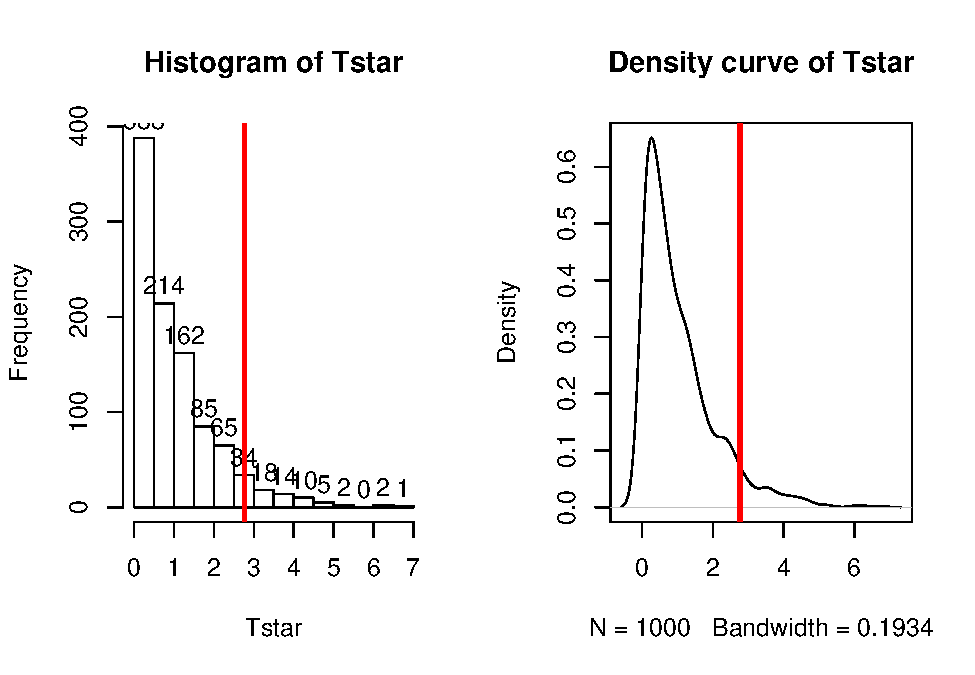
\includegraphics{03-oneWayAnova_files/figure-latex/Figure3-7-1.pdf}
\caption{\label{fig:Figure3-7}Histogram and density curve of the permutation distribution
of the F-statistic with bold, vertical line for observed value of the
test statistic of 2.77.}
\end{figure}

The permutation-based p-value is 0.064 which, again, matches the other
results closely. The first conclusion is that using a test statistic of
either the \(F\)-statistic or the \(\text{SS}_A\) provide similar
permutation results. However, we tend to favor using the \(F\)-statistic
because it is more commonly used in reporting ANOVA results, not because
it is any better in a permutation context.

It is also interesting to compare the permutation distribution for the
\(F\)-statistic and the parametric \(F(2, 111)\) distribution (Figure
\ref{fig:Figure3-8}). They do not match perfectly but are quite similar.
Some the differences around 0 are due to the behavior of the method used
to create the density curve and are not really a problem for the
methods. The similarity in the two curves explains why both methods give
similar results. In some situations, the correspondence will not be
quite so close.




\begin{figure}
\centering
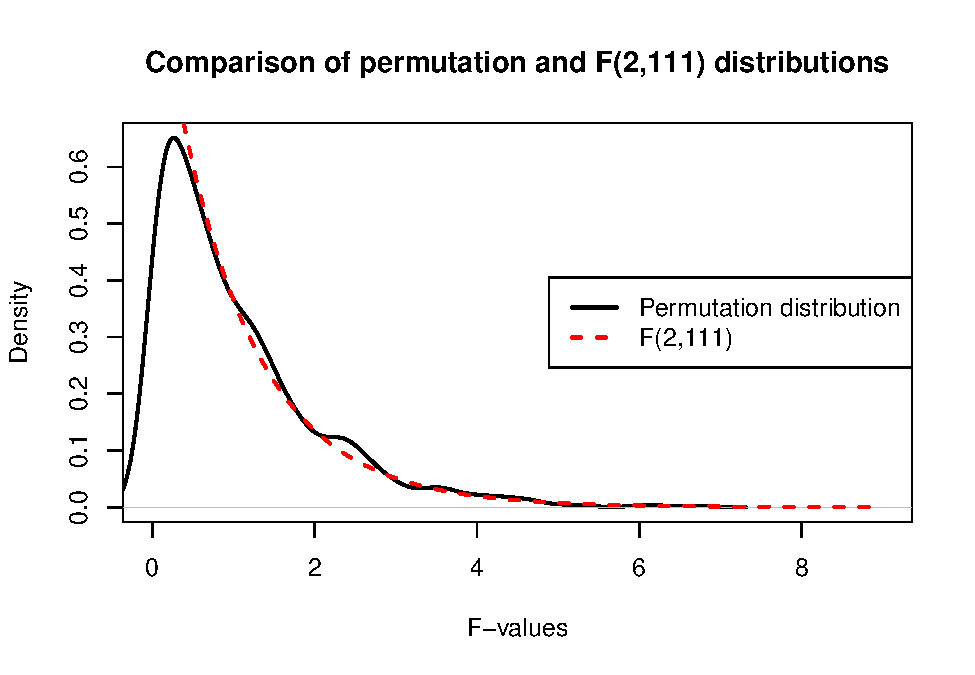
\includegraphics{03-oneWayAnova_files/figure-latex/Figure3-8-1.pdf}
\caption{\label{fig:Figure3-8}Comparison of \(F(2, 111)\) (dashed line) and permutation
distribution (solid line).}
\end{figure}

So how can we rectify this result (\(\text{p-value}\approx 0.06\)) and
the Chapter \ref{chapter2} result that detected a difference between
\emph{Average} and \emph{Unattractive} with a
\(\text{p-value}\approx 0.03\)? I selected the two groups to compare in
Chapter \ref{chapter2} because they were furthest apart.
``Cherry-picking'' the comparison that is likely to be most different
creates a false sense of the real situation and inflates the Type I
error rate because of the selection. If the entire suite of pairwise
comparisons are considered, this result may lose some of its luster. In
other words, if we consider the suite of three pair-wise differences
(and the tests) implicit in comparing all of them, we may need stronger
evidence in the most different pair than a p-value of 0.033 to suggest
overall differences. In this situation, the \emph{Beautiful} and
\emph{Average} groups are not that different from each other so their
difference does not contribute much to the will revisit this topic and
consider a method that is statistically valid for performing all
possible pair-wise comparisons that is also consistent with our overall
test results.

\section{ANOVA model diagnostics including QQ-plots}\label{section3-4}

The requirements for a One-Way ANOVA \(F\)-test are similar to those
discussed in Chapter \ref{chapter2}, except that there are now \(J\)
groups instead of only 2. Specifically, the linear model assumes:

\begin{enumerate}
\def\labelenumi{\arabic{enumi}.}
\item
  \textbf{Independent observations},
\item
  \textbf{Equal variances}, and
\item
  \textbf{Normal distributions}.
\end{enumerate}

For assessing equal variances across the groups, it is best to use plots
to assess this. We can use boxplots and beanplots to compare the spreads
of the groups, which were provided in Figure \ref{fig:Figure3-1}. The
range and IQRs should be relatively similar across the groups if you do
not find evidence of a problem with this assumption. You should start
with noting how clear or big the violation of the assumption might be
but remember that there will always be some differences in the variation
among groups even if the true variability is exactly equal in the
populations. In addition to our direct plotting, there are some
diagnostic plots available from the \texttt{lm} function that can help
us more clearly assess potential violations of the previous assumptions.

We can obtain a suite of four diagnostic plots by using the
\texttt{plot} function on any linear model object that we have fit. To
get all the plots together in four panels we need to add the
\texttt{par(mfrow=c(2,\ 2))} command to tell R to make a graph with 4
panels\footnote{We have been using this function quite a bit to make
  multi-panel graphs but did not show you that line of code. But you
  need to use this command for linear model diagnostics or you won't get
  the plots we want from the model. And you really just need
  \texttt{plot(lm2)} but the \texttt{pch=16} option makes it easier to
  see some of the points in the plots.}.

\begin{Shaded}
\begin{Highlighting}[]
\KeywordTok{par}\NormalTok{(}\DataTypeTok{mfrow=}\KeywordTok{c}\NormalTok{(}\DecValTok{2}\NormalTok{,}\DecValTok{2}\NormalTok{))}
\KeywordTok{plot}\NormalTok{(lm2,}\DataTypeTok{pch=}\DecValTok{16}\NormalTok{)}
\end{Highlighting}
\end{Shaded}

There are two plots in Figure \ref{fig:Figure3-9} with useful
information for the equal variance assumption. The ``Residuals vs
Fitted'' panel in the top left displays the residuals
\((e_{ij} = y_{ij}-\hat{y}_ij)\) on the y-axis and the fitted values
\((\hat{y}_{ij})\) on the x-axis. This allows you to see if the
variability of the observations differs across the groups as a function
of the mean of the groups because all the observations in the same group
get the same fitted value, the mean of the group. In this plot, the
points seem to have fairly similar spreads at the fitted values for the
three groups with fitted values of 4, 4.3, and 6. The ``Scale-Location''
plot in the lower left panel has the same x-axis but the y-axis contains
the square-root of the absolute value of the standardized residuals. The
absolute value transforms all the residuals into a magnitude scale
(removing direction) and the square-root helps you see differences in
variability more accurately. The standardization scales them to have a
variance of 1 so help you in other displays to get a sense of how many
standard deviations you are away from the mean in the residual
distribution. The visual assessment is similar in the two plots -- you
want to consider whether it appears that the groups have somewhat
similar or noticeably different amounts of variability. If you see a
clear funnel shape in the Residuals vs Fitted or an increase or decrease
in the upper edge of points in the Scale-Location plot that may indicate
a violation of the constant variance assumption. Remember that some
variation across the groups is expected and is OK, but large differences
in spreads are problematic for all the procedures that involve linear
models. When discussing these results, you want to discuss how clearly
the differences in variation are and whether that \emph{shows a clear
violation of the assumption} of equal variance for all observations.
Like in hypothesis testing, you can't prove that you've met assumptions
based on a plot ``looking OK'', but you can say that there is no clear
evidence that the assumption is violated!



\begin{figure}
\centering
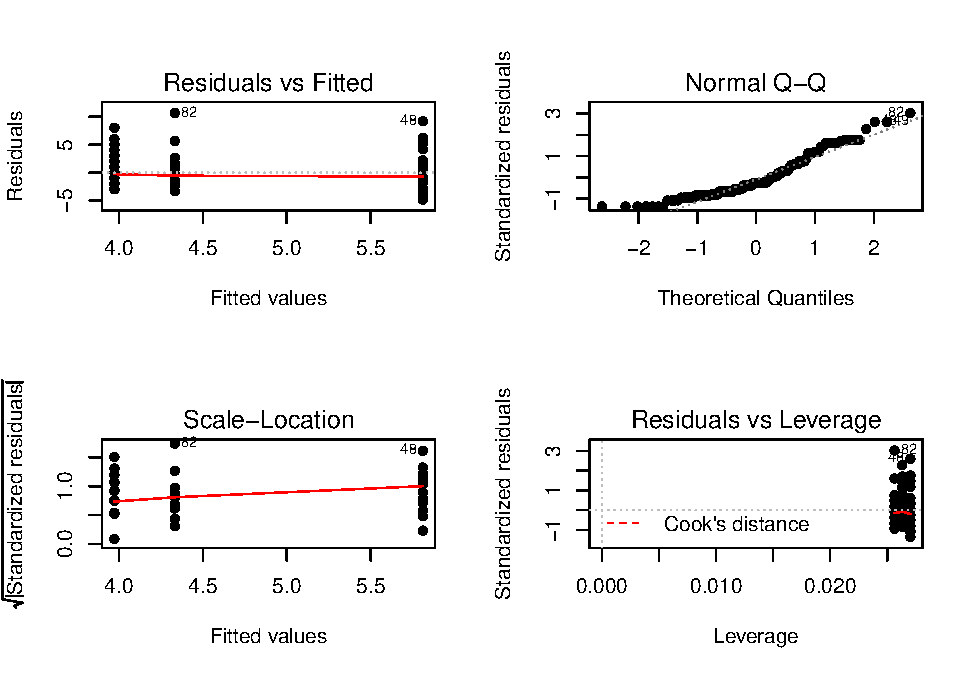
\includegraphics{03-oneWayAnova_files/figure-latex/Figure3-9-1.pdf}
\caption{\label{fig:Figure3-9}Default diagnostic plots for the linear model.}
\end{figure}

The linear model assumes that all the random errors
(\(\varepsilon_{ij}\)) follow a normal distribution. To gain insight
into the validity of this assumption, we can explore the original
observations as displayed in the beanplots, mentally subtracting off the
differences in the means and focusing on the shapes of the distributions
of observations in each group. These plots are especially good for
assessing whether there is there a skew or outliers present in each
group. If so, by definition, the normality assumption is violated. But
our assumption is about the distribution of all the errors after the
remove the differences in the means and so we want an overall assessment
technique to understand how reasonable our assumption is overall for our
model. The residuals from the entire model provide us with estimates of
the random errors and if the normality assumption is met, then the
residuals all-together should approximately follow a normal
distribution. The \textbf{\emph{Normal Q-Q Plot}} in upper right panel
of Figure \ref{fig:Figure3-9} is a direct visual assessment of how well
our residuals match what we would expect from a normal distribution.
Outliers, skew, heavy and light-tailed aspects of distributions (all
violations of normality) show up in this plot once you learn to read it
-- which is our next task. To make it easier to read QQ-plots, it is
nice to start with just considering histograms and/or density plots of
the residuals and to see how that maps into this new display. We can
obtain the residuals from the linear model using the \texttt{residuals}
function on any linear model object.




\begin{Shaded}
\begin{Highlighting}[]
\KeywordTok{par}\NormalTok{(}\DataTypeTok{mfrow=}\KeywordTok{c}\NormalTok{(}\DecValTok{1}\NormalTok{,}\DecValTok{2}\NormalTok{))}
\NormalTok{eij<-}\KeywordTok{residuals}\NormalTok{(lm2)}
\KeywordTok{hist}\NormalTok{(eij, }\DataTypeTok{main=}\StringTok{"Histogram of residuals"}\NormalTok{)}
\KeywordTok{plot}\NormalTok{(}\KeywordTok{density}\NormalTok{(eij), }\DataTypeTok{main=}\StringTok{"Density plot of residuals"}\NormalTok{, }\DataTypeTok{ylab=}\StringTok{"Density"}\NormalTok{,}
     \DataTypeTok{xlab=}\StringTok{"Residuals"}\NormalTok{)}
\end{Highlighting}
\end{Shaded}

\begin{figure}
\centering
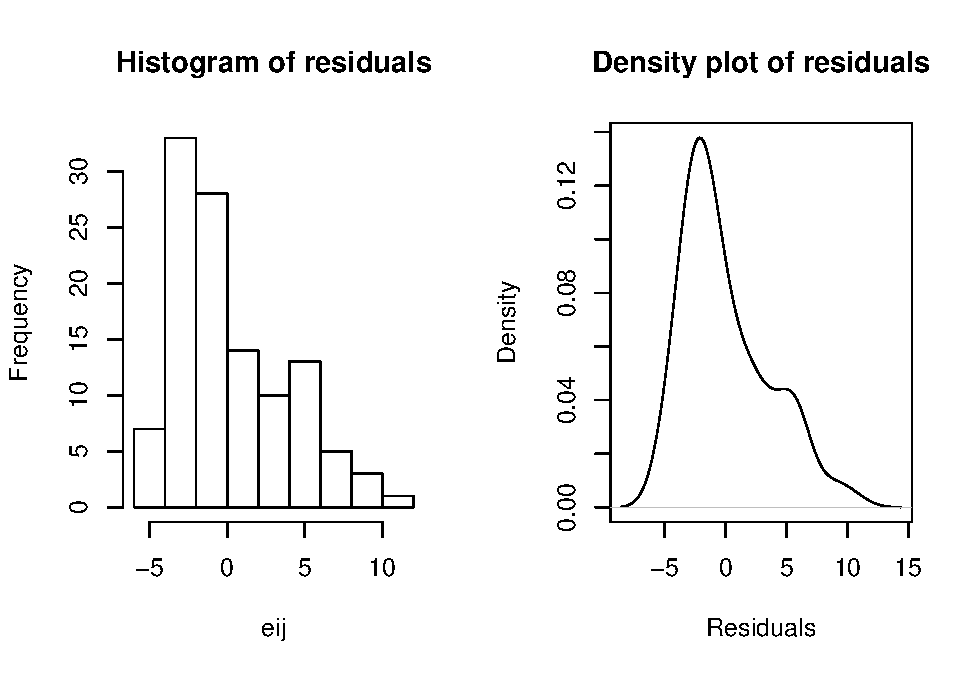
\includegraphics{03-oneWayAnova_files/figure-latex/Figure3-10-1.pdf}
\caption{\label{fig:Figure3-10}Histogram and density curve of the linear model raw
residuals.}
\end{figure}

Figure \ref{fig:Figure3-10} shows that there is a right skew present in
the residuals for the prisoner rating data model that accounted for
different means in the three groups, which is consistent with the
initial assessment of some right skew in the plots of observations in
each group.

A Quantile-Quantile plot (\textbf{\emph{QQ-plot}}) shows the ``match''
of an observed distribution with a theoretical distribution, almost
always the normal distribution. They are also known as Quantile
Comparison, Normal Probability, or Normal Q-Q plots, with the last two
names being specific to comparing results to a normal distribution. In
this version\footnote{Along with multiple names, there is variation of
  what is plotted on the x and y axes and the scaling of the values
  plotted, increasing the challenge of interpreting QQ-plots. We are
  consistent about the x and y axis choices but different functions that
  make these plots in R do switch the axes.}, the QQ-plots display the
value of observed percentiles in the residual distribution on the y-axis
versus the percentiles of a theoretical normal distribution on the
x-axis. If the observed \textbf{distribution of the residuals matches
the shape of the normal distribution, then the plotted points should
follow a 1-1 relationship.} If the points follow the displayed straight
line then that suggests that the residuals have a similar shape to a
normal distribution. Some variation is expected around the line and some
patterns of deviation are worse than others for our models, so you need
to go beyond saying ``it does not match a normal distribution''. It is
best to be specific about the type of deviation you are detecting. And
to do that, we need to practice interpreting some QQ-plots.

The QQ-plot of the linear model residuals from Figure
\ref{fig:Figure3-9} is extracted and enhanced it a little to make Figure
\ref{fig:Figure3-11} so we can just focus on it. We know from looking at
the histogram that this is a slightly right skewed distribution. The
QQ-plot places the observed \textbf{\emph{standardized}}\footnote{Here
  this means re-scaled so that they should have similar scaling to a
  standard normal with mean 0 and standard deviation 1. This does not
  change the shape of the distribution but can make outlier
  identification simpler -- having a standardized residual more extreme
  than 5 or -5 would suggest a deviation from normality since we rarely
  see values that many standard deviations from the mean in a normal
  distribution. But mainly focus on the shape of the pattern in the
  QQ-plot.} \textbf{\emph{residuals}} on the y-axis and the theoretical
normal values on the x-axis. The most noticeable deviation from the 1-1
line is in the lower left corner of the plot. These are for the negative
residuals (left tail) and there are many residuals at around the same
value that are a little smaller than -1. If the distribution had
followed the normal distribution here, the points would be on the 1-1
line and there would be some standardized residuals much smaller than
-1.5. So we are not getting as much spread in the smaller residuals as
we would expect in a normal distribution. If you go back to the
histogram you can see that the smallest residuals are all stacked up and
do not spread out like the left tail of a normal distribution should. In
the right tail (positive) residuals, there is also a systematic lifting
from the 1-1 line to larger values in the residuals than the normal
would generate. For example, the point labeled as ``82'' (the 82nd
observation in the data set) has a value of 3 in residuals but should
actually be smaller (maybe 2.5) if the distribution was normal. Put
together, this pattern in the QQ-plot suggests that the left tail is too
compacted (too short) and the right tail is too spread out -- this is
the right skew we identified from the histogram and density curve!



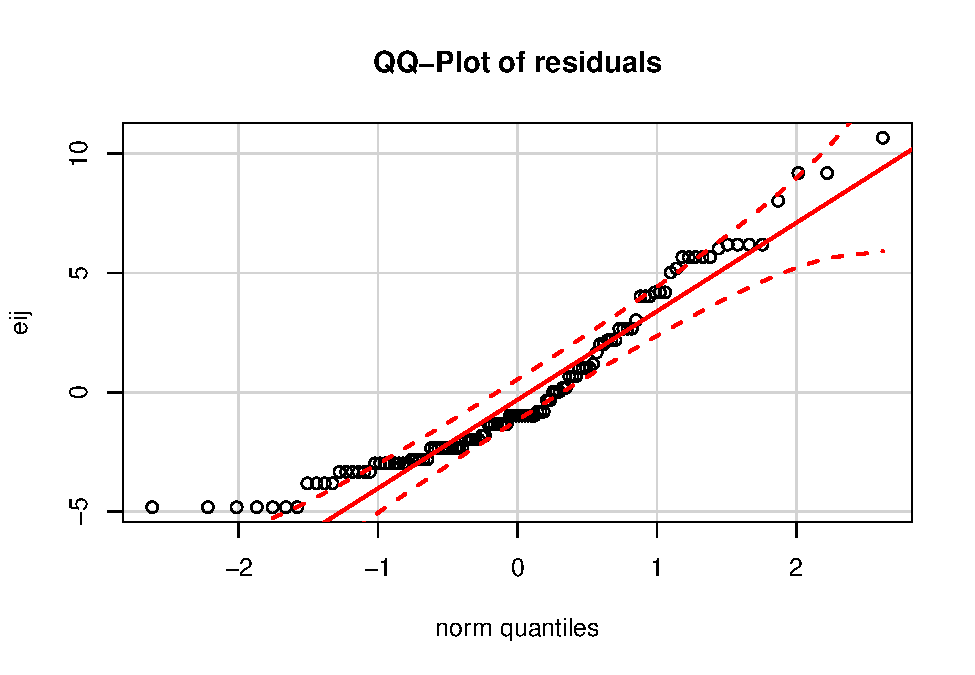
\includegraphics{03-oneWayAnova_files/figure-latex/Figure3-11-1.pdf}
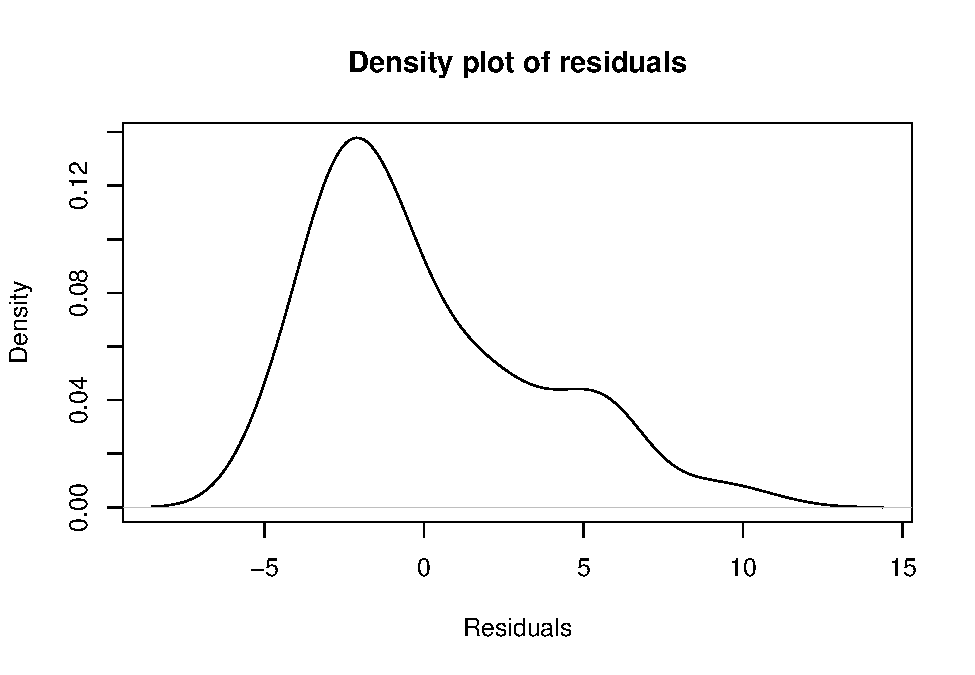
\includegraphics{03-oneWayAnova_files/figure-latex/Figure3-11-2.pdf}

Generally, when both tails deviate on the same side of the line (forming
a sort of quadratic curve, especially in more extreme cases), that is
evidence of a skew. To see some different potential shapes in QQ-plots,
six different data sets are displayed in Figures \ref{fig:Figure3-12}
and \ref{fig:Figure3-13}. In each row, a QQ-plot and associated density
curve are displayed. If the points are both above the 1-1 line in the
lower and upper tails as in Figure \ref{fig:Figure3-12}(a), then the
pattern is a right skew, here even more extreme than in the real data
set. If the points are below the 1-1 line in both tails as in Figure
\ref{fig:Figure3-12}(c), then the pattern is identified as a left skew.
Skewed residual distributions (either direction) are problematic for
models that assume normally distributed responses but not necessarily
for our permutation approaches if all the groups have similar skewed
shapes. The other problematic pattern is to have more spread than a
normal curve as in Figure \ref{fig:Figure3-12}(e) and (f). This shows up
with the points being below the line in the left tail (more extreme
negative than expected by the normal) and the points being above the
line for the right tail (more extreme positive than the normal
predicts). We call these distributions \textbf{\emph{heavy-tailed}}
which can manifest as distributions with outliers in both tails or just
a bit more spread out than a normal distribution. Heavy-tailed residual
distributions can be problematic for our models as the variation is
greater than what the normal distribution can account for and our
methods might under-estimate the variability in the results. The
opposite pattern with the left tail above the line and the right tail
below the line suggests less spread (\textbf{\emph{lighter-tailed}})
than a normal as in Figure \ref{fig:Figure3-12}(g) and (h). This pattern
is relatively harmless and you can proceed with methods that assume
normality safely as they will just be a little conservative.




\begin{figure}
\centering
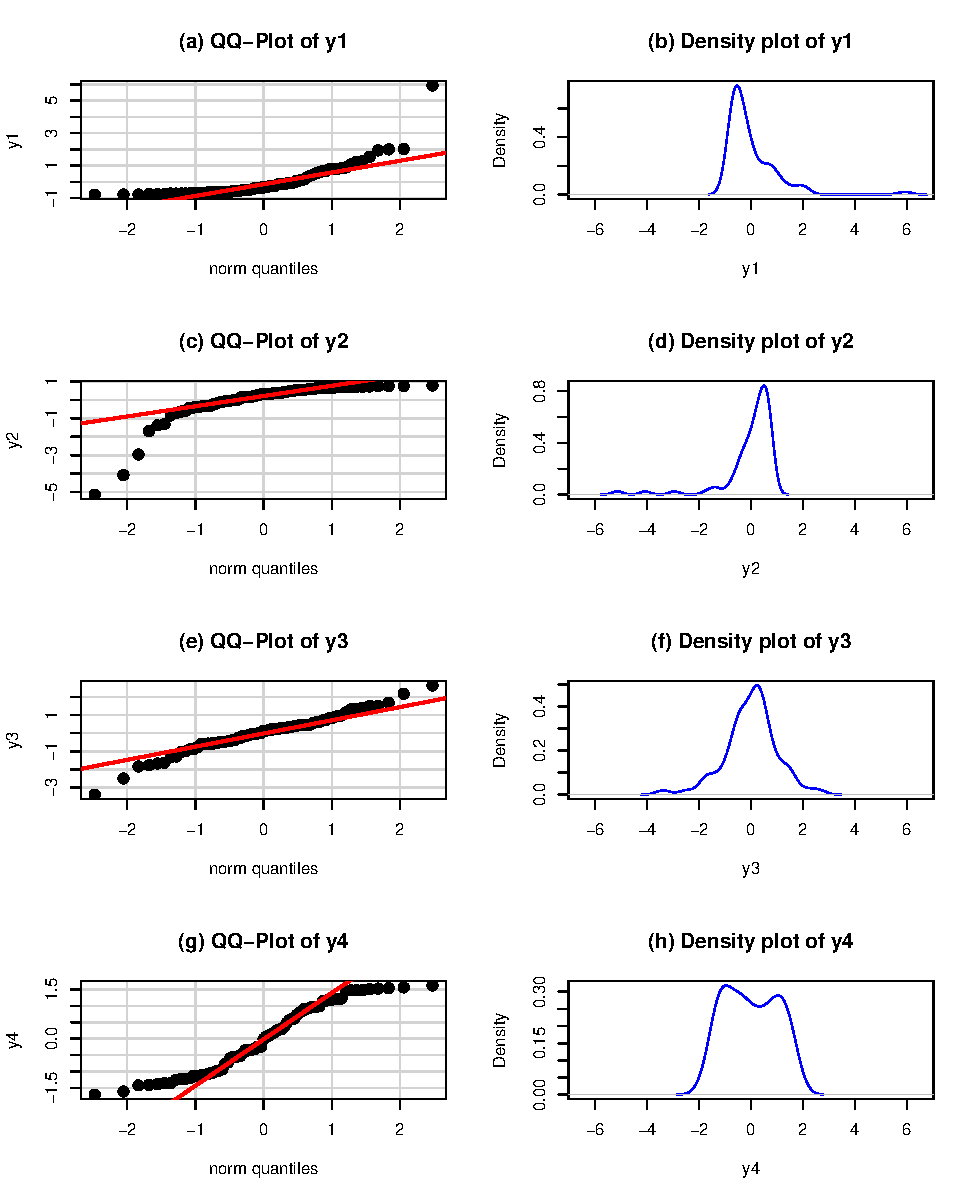
\includegraphics{03-oneWayAnova_files/figure-latex/Figure3-12-1.pdf}
\caption{\label{fig:Figure3-12}QQ-plots and density curves of four simulated
distributions with different shapes.}
\end{figure}

Finally, to help you calibrate expectations for data that are actually
normally distributed, two data sets simulated from normal distributions
are displayed in Figure \ref{fig:Figure3-13}. Note how neither follows
the line exactly but that the overall pattern matches fairly well.
\textbf{You have to allow for some variation from the line in real data
sets} and focus on when there are really noticeable issues in the
distribution of the residuals such as those displayed above. Again, you
will never be able to prove that you have normally distributed residuals
even if the residuals are all exactly on the line, but if you see
QQ-plots as in Figure \ref{fig:Figure3-12} you can encounter situations
that provide evidence of clear violations of the normality assumption.




\begin{figure}
\centering
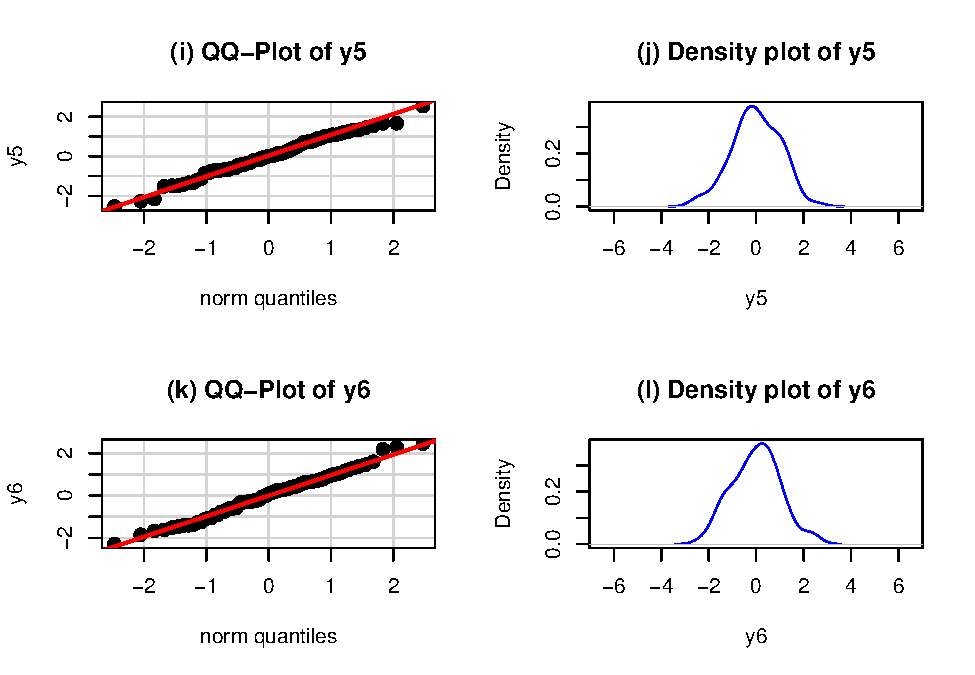
\includegraphics{03-oneWayAnova_files/figure-latex/Figure3-13-1.pdf}
\caption{\label{fig:Figure3-13}Two more simulated data sets, generated from normal
distributions.}
\end{figure}

The last issues with assessing the assumptions in an ANOVA relates to
situations where the methods are more or less
\textbf{\emph{resistant}}\footnote{A resistant procedure is one that is
  not severely impacted by a particular violation of an assumption. For
  example, the median is resistant to the impact of an outlier.} to
violations of assumptions. For reasons beyond the scope of this book,
the parametric ANOVA F-test is more resistant to violations of the
assumptions of the normality and equal variance assumptions if the
design is balanced. A \textbf{\emph{balanced design}} occurs when each
group is measured the same number of times. The resistance decreases as
the data set becomes less balanced, as the sample sizes in the groups
are more different, so having close to balance is preferred to a more
imbalanced situation if there is a choice available. There is some
intuition available here -- it makes some sense that you would have
better results in comparing groups if the information available is
similar in all the groups and none are relatively under-represented. We
can check the number of observations in each group to see if they are
equal or similar using the \texttt{tally} function from the
\texttt{mosaic} package. This function is useful for being able to get
counts of observations, especially for cross-classifying observations on
two variables that is used in Chapter \ref{chapter5}. For just a single
variable, we use \texttt{tally(\textasciitilde{}x,\ data=...)}:

\begin{Shaded}
\begin{Highlighting}[]
\KeywordTok{require}\NormalTok{(mosaic)}
\KeywordTok{tally}\NormalTok{(}\OperatorTok{~}\NormalTok{Attr, }\DataTypeTok{data=}\NormalTok{MockJury)}
\end{Highlighting}
\end{Shaded}

\begin{verbatim}
## Attr
##    Beautiful      Average Unattractive 
##           39           38           37
\end{verbatim}

So the sample sizes do vary among the groups and the design is
technically not balanced, but it is also very close to being balanced
with only two more observations in the largest group compared to the
smallest group size. This tells us that the \(F\)-test should have some
resistance to violations of assumptions. This nearly balanced design,
and the moderate sample size (over 37 per group is considered a good but
not large sample), make the parametric and nonparametric approaches
provide similar results in this data set even in the presence of the
skewed residual error distribution.

\section{Guinea pig tooth growth One-Way ANOVA
example}\label{section3-5}

A second example of the One-way ANOVA methods involves a study of length
of odontoblasts (cells that are responsible for tooth growth) in 60
Guinea Pigs (measured in microns) from \citet{Crampton1947}. \(N=60\)
Guinea Pigs were obtained from a local breeder and each received one of
three dosages (0.5, 1, or 2 mg/day) of Vitamin C via one of two delivery
methods, Orange Juice (\emph{OJ}) or ascorbic acid (the stuff in vitamin
C capsules, called \(VC\) below) as the source of Vitamin C in their
diets. Each guinea pig was randomly assigned to receive one of the six
different treatment combinations possible (OJ at 0.5 mg, OJ at 1 mg, OJ
at 2 mg, VC at 0.5 mg, VC at 1 mg, and VC at 2 mg). The animals were
treated similarly otherwise and we can assume lived in separate cages
and only one observation was taken for each guinea pig, so we can assume
the observations are independent. We need to create a variable that
combines the levels of delivery type (OJ, VC) and the dosages (0.5, 1,
and 2) to use our One-Way ANOVA on the six levels. The
\texttt{interaction} function can be used create a new variable that is
based on combinations of the levels of other variables. Here a new
variable is created in the \texttt{ToothGrowth} data.frame that we
called \texttt{Treat} that provides a six-level grouping variable for
our One-Way ANOVA to compare the combinations of treatments. To get a
sense of the pattern of observations in the data set, the counts in
\texttt{supp} (supplement type) and \texttt{dose} are provided.

\begin{Shaded}
\begin{Highlighting}[]
\KeywordTok{data}\NormalTok{(ToothGrowth) }\CommentTok{#Available in Base R}
\KeywordTok{require}\NormalTok{(mosaic)}
\KeywordTok{tally}\NormalTok{(}\OperatorTok{~}\NormalTok{supp,}\DataTypeTok{data=}\NormalTok{ToothGrowth) }\CommentTok{#Supplement Type (VC or OJ)}
\end{Highlighting}
\end{Shaded}

\begin{verbatim}
## supp
## OJ VC 
## 30 30
\end{verbatim}

\begin{Shaded}
\begin{Highlighting}[]
\KeywordTok{tally}\NormalTok{(}\OperatorTok{~}\NormalTok{dose,}\DataTypeTok{data=}\NormalTok{ToothGrowth) }\CommentTok{#Dosage level}
\end{Highlighting}
\end{Shaded}

\begin{verbatim}
## dose
## 0.5   1   2 
##  20  20  20
\end{verbatim}

\begin{Shaded}
\begin{Highlighting}[]
\CommentTok{#Creates a new variable Treat with 6 levels}
\NormalTok{ToothGrowth}\OperatorTok{$}\NormalTok{Treat=}\KeywordTok{with}\NormalTok{(ToothGrowth,}\KeywordTok{interaction}\NormalTok{(supp,dose)) }

\CommentTok{#New variable that combines supplement type and dosage}
\KeywordTok{tally}\NormalTok{(}\OperatorTok{~}\NormalTok{Treat,}\DataTypeTok{data=}\NormalTok{ToothGrowth) }
\end{Highlighting}
\end{Shaded}

\begin{verbatim}
## Treat
## OJ.0.5 VC.0.5   OJ.1   VC.1   OJ.2   VC.2 
##     10     10     10     10     10     10
\end{verbatim}

The \texttt{tally} function helps us to check for balance; this is a
balanced design because the same number of guinea pigs
(\(n_j=10 \text{ for } j=1, 2,\ldots, 6\)) were measured in each
treatment combination.

With the variable \texttt{Treat} prepared, the first task is to
visualize the results using boxplots and beanplots\footnote{Note that to
  see all the group labels in the plot when making the figure, you have
  to widen the plot window before copying the figure out of R. You can
  resize the plot window using the small vertical and horizontal ``=''
  signs in the grey bars that separate the different panels in RStudio.}
(Figure \ref{fig:Figure3-14}) and generate some summary statistics for
each group using \texttt{favstats}.




\begin{Shaded}
\begin{Highlighting}[]
\KeywordTok{par}\NormalTok{(}\DataTypeTok{mfrow=}\KeywordTok{c}\NormalTok{(}\DecValTok{1}\NormalTok{,}\DecValTok{2}\NormalTok{))}
\KeywordTok{boxplot}\NormalTok{(len}\OperatorTok{~}\NormalTok{Treat,}\DataTypeTok{data=}\NormalTok{ToothGrowth,}\DataTypeTok{ylab=}\StringTok{"Tooth Growth in microns"}\NormalTok{)}
\KeywordTok{beanplot}\NormalTok{(len}\OperatorTok{~}\NormalTok{Treat,}\DataTypeTok{data=}\NormalTok{ToothGrowth,}\DataTypeTok{log=}\StringTok{""}\NormalTok{,}\DataTypeTok{col=}\StringTok{"yellow"}\NormalTok{,}
         \DataTypeTok{method=}\StringTok{"jitter"}\NormalTok{,}\DataTypeTok{ylab=}\StringTok{"Tooth Growth in microns"}\NormalTok{)}
\end{Highlighting}
\end{Shaded}

\begin{figure}
\centering
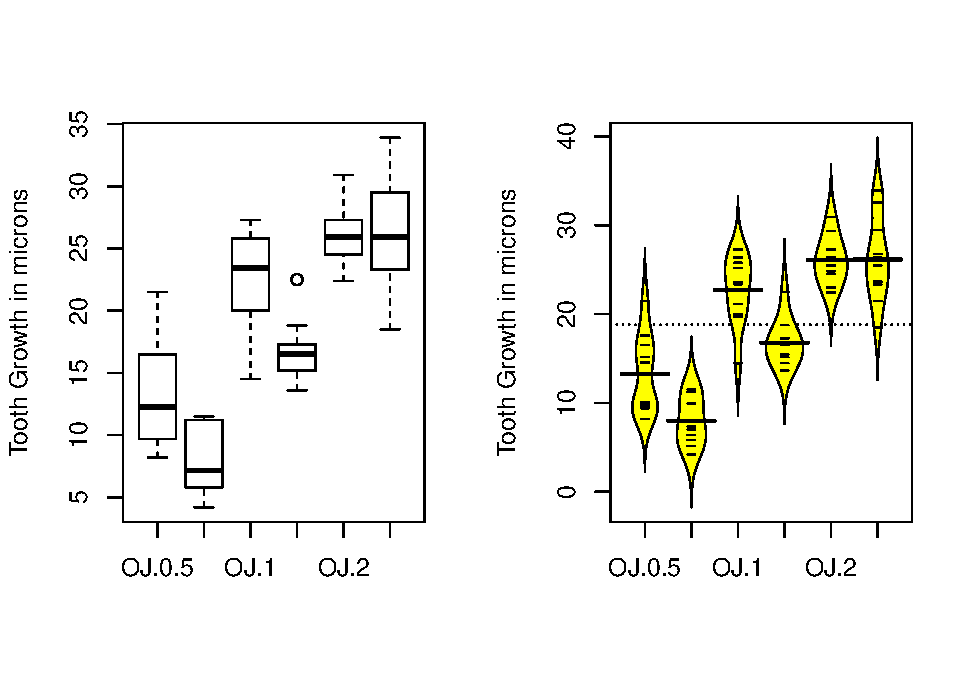
\includegraphics{03-oneWayAnova_files/figure-latex/Figure3-14-1.pdf}
\caption{\label{fig:Figure3-14}Boxplot and beanplot of tooth growth responses for the six
treatment level combinations.}
\end{figure}

\begin{Shaded}
\begin{Highlighting}[]
\KeywordTok{favstats}\NormalTok{(len}\OperatorTok{~}\NormalTok{Treat,}\DataTypeTok{data=}\NormalTok{ToothGrowth)}
\end{Highlighting}
\end{Shaded}

\begin{verbatim}
##    Treat  min     Q1 median     Q3  max  mean       sd  n missing
## 1 OJ.0.5  8.2  9.700  12.25 16.175 21.5 13.23 4.459709 10       0
## 2 VC.0.5  4.2  5.950   7.15 10.900 11.5  7.98 2.746634 10       0
## 3   OJ.1 14.5 20.300  23.45 25.650 27.3 22.70 3.910953 10       0
## 4   VC.1 13.6 15.275  16.50 17.300 22.5 16.77 2.515309 10       0
## 5   OJ.2 22.4 24.575  25.95 27.075 30.9 26.06 2.655058 10       0
## 6   VC.2 18.5 23.375  25.95 28.800 33.9 26.14 4.797731 10       0
\end{verbatim}

Figure \ref{fig:Figure3-14} suggests that the mean tooth growth
increases with the dosage level and that OJ might lead to higher growth
rates than VC except at a dosage of 2 mg/day. The variability around the
means looks to be small relative to the differences among the means, so
we should expect a small p-value from our \(F\)-test. The design is
balanced as noted above (\(n_j=10\) for all six groups) so the methods
are some what resistant to impacts from non-normality and non-constant
variance. There is some suggestion of non-constant variance in the plots
but this will be explored further below when we can remove the
difference in the means and combine all the residuals together. There
might be some skew in the responses in some of the groups but there are
only 10 observations per group so skew in the boxplots could be
generated by impacts of very few of the observations.

Now we can apply our 6+ steps for performing a hypothesis test with
these observations. The initial step is deciding on the claim to be
assessed and the test statistic to use. This is a six group situation
with a quantitative response, identifying it as a One-Way ANOVA where we
want to test a null hypothesis that all the groups have the same
population mean, at least to start. We will use a 5\% significance
level.

\begin{enumerate}
\def\labelenumi{\arabic{enumi}.}
\item
  \textbf{Hypotheses}:
  \(\boldsymbol{H_0: \mu_{OJ0.5} = \mu_{VC0.5} = \mu_{OJ1} = \mu_{VC1} = \mu_{OJ2} = \mu_{VC2}} \textbf{ vs }\)
  \(\boldsymbol{H_A:} \textbf{ Not all } \boldsymbol{\mu_j} \textbf{ equal}\)

  \begin{itemize}
  \item
    The null hypothesis could also be written in reference-coding as
    below since OJ.0.5 is chosen as the baseline group (discussed
    below).

    \begin{itemize}
    \tightlist
    \item
      \(\boldsymbol{H_0:\tau_{VC0.5}=\tau_{OJ1}=\tau_{VC1}=\tau_{OJ2}=\tau_{VC2}=0}\)
    \end{itemize}
  \item
    The alternative hypothesis can be left a bit less specific:

    \begin{itemize}
    \tightlist
    \item
      \(\boldsymbol{H_A:} \textbf{ Not all } \boldsymbol{\tau_j} \textbf{ equal 0}\)
    \end{itemize}
  \end{itemize}
\item
  \textbf{Validity conditions}:

  \begin{itemize}
  \item
    Independence:

    \begin{itemize}
    \tightlist
    \item
      This is where the separate cages note above is important. Suppose
      that there were cages that contained multiple animals and they
      competed for food or could share illness or levels of activity.
      The animals in one cage might be systematically different from the
      others and this ``clustering'' of observations would present a
      potential violation of the independence assumption. If the
      experiment had the animals in separate cages, there is no clear
      dependency in the design of the study and we can assume that there
      is no problem with this assumption.
    \end{itemize}
  \item
    Constant variance:

    \begin{itemize}
    \tightlist
    \item
      As noted above, there is some indication of a difference in the
      variability among the groups in the boxplots and beanplots but the
      sample size was small in each group. We need to fit the linear
      model to get the other diagnostic plots to make an overall
      assessment.
    \end{itemize}

    (ref:fig3-15) Diagnostic plots for the toothgrowth model.

\begin{Shaded}
\begin{Highlighting}[]
\NormalTok{m2<-}\KeywordTok{lm}\NormalTok{(len}\OperatorTok{~}\NormalTok{Treat,}\DataTypeTok{data=}\NormalTok{ToothGrowth)}
\KeywordTok{par}\NormalTok{(}\DataTypeTok{mfrow=}\KeywordTok{c}\NormalTok{(}\DecValTok{2}\NormalTok{,}\DecValTok{2}\NormalTok{))}
\KeywordTok{plot}\NormalTok{(m2,}\DataTypeTok{pch=}\DecValTok{16}\NormalTok{)}
\end{Highlighting}
\end{Shaded}

    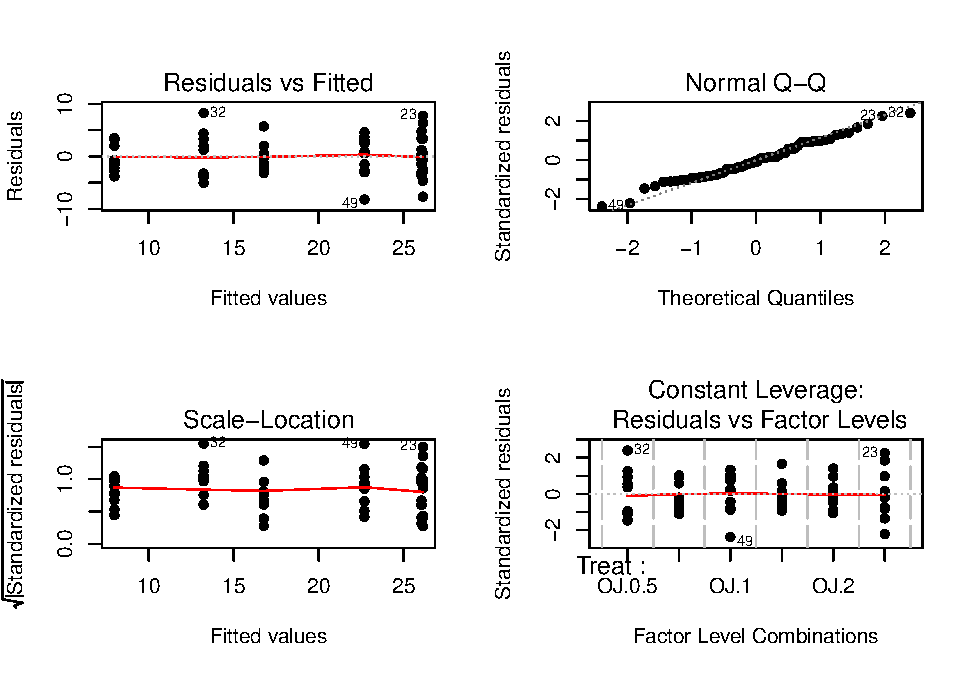
\includegraphics{03-oneWayAnova_files/figure-latex/Figure3-15-1.pdf}

    \begin{itemize}
    \item
      The Residuals vs Fitted panel in Figure \ref{fig:Figure3-15} shows
      some difference in the spreads but the spread is not that
      different between the groups.
    \item
      The Scale-Location plot also shows just a little less variability
      in the group with the smallest fitted value but the spread of the
      groups looks fairly similar in this alternative scaling.
    \item
      Put together, the evidence for non-constant variance is not that
      strong and we can assume that there is at least not a major
      problem with this assumption.
    \end{itemize}
  \item
    Normality of residuals:

    \begin{itemize}
    \tightlist
    \item
      The Normal Q-Q plot shows a small deviation in the lower tail but
      nothing that we wouldn't expect from a normal distribution. So
      there is no evidence of a problem with the normality assumption in
      the upper right panel of Figure \ref{fig:Figure3-15}.
    \end{itemize}
  \end{itemize}
\item
  \textbf{Calculate the test statistic}:

  \begin{itemize}
  \tightlist
  \item
    The ANOVA table for our model follows, providing an \(F\)-statistic
    of 41.557:
  \end{itemize}

\begin{Shaded}
\begin{Highlighting}[]
\KeywordTok{anova}\NormalTok{(m2)}
\end{Highlighting}
\end{Shaded}

\begin{verbatim}
## Analysis of Variance Table
## 
## Response: len
##           Df  Sum Sq Mean Sq F value    Pr(>F)
## Treat      5 2740.10  548.02  41.557 < 2.2e-16
## Residuals 54  712.11   13.19
\end{verbatim}
\item
  \textbf{Find the p-value}:

  \begin{itemize}
  \item
    There are two options here, especially since it seems that our
    assumptions about variance and normality are not violated (note that
    we do not say ``met'' -- we just have no clear evidence against
    them). The parametric and nonparametric approaches should provide
    similar results here.
  \item
    The parametric approach is easiest -- the p-value comes from the
    previous ANOVA table as \texttt{\textless{}2e-16}. First, note that
    this is in scientific notation that is a compact way of saying that
    the p-value here is \(2.2*10^{-16}\) or 0.00000000000000022. When
    you see \texttt{2.2e-16} in R output, it also means that the
    calculation is at the numerical precision of the computer. What R is
    really trying to report is that this is a very small number.
    \textbf{When you encounter p-values that are smaller than 0.0001,
    you should just report that the p-value\textless{}0.0001} Do not
    report that it is 0 as this gives the false impression that there is
    no chance of the result occurring when it is just a really small
    probability. This distribution (the distribution of the test
    statistic if the null hypothesis is true).
  \item
    The nonparametric approach is not too hard so we can compare the two
    approaches here as well:
  \end{itemize}

  (ref:fig3-16) Histogram and density curve of permutation distribution
  for \(F\)-statistic for tooth growth data. Observed test statistic in
  bold, vertical line at 41.56.

\begin{Shaded}
\begin{Highlighting}[]
\NormalTok{Tobs <-}\StringTok{ }\KeywordTok{anova}\NormalTok{(}\KeywordTok{lm}\NormalTok{(len}\OperatorTok{~}\NormalTok{Treat,}\DataTypeTok{data=}\NormalTok{ToothGrowth))[}\DecValTok{1}\NormalTok{,}\DecValTok{4}\NormalTok{]; Tobs}
\end{Highlighting}
\end{Shaded}

\begin{verbatim}
## [1] 41.55718
\end{verbatim}

\begin{Shaded}
\begin{Highlighting}[]
\KeywordTok{par}\NormalTok{(}\DataTypeTok{mfrow=}\KeywordTok{c}\NormalTok{(}\DecValTok{1}\NormalTok{,}\DecValTok{2}\NormalTok{))}
\NormalTok{B<-}\StringTok{ }\DecValTok{1000}
\NormalTok{Tstar<-}\KeywordTok{matrix}\NormalTok{(}\OtherTok{NA}\NormalTok{,}\DataTypeTok{nrow=}\NormalTok{B)}
\ControlFlowTok{for}\NormalTok{ (b }\ControlFlowTok{in}\NormalTok{ (}\DecValTok{1}\OperatorTok{:}\NormalTok{B))\{}
\NormalTok{  Tstar[b]<-}\KeywordTok{anova}\NormalTok{(}\KeywordTok{lm}\NormalTok{(len}\OperatorTok{~}\KeywordTok{shuffle}\NormalTok{(Treat),}\DataTypeTok{data=}\NormalTok{ToothGrowth))[}\DecValTok{1}\NormalTok{,}\DecValTok{4}\NormalTok{]}
\NormalTok{\}}
\KeywordTok{pdata}\NormalTok{(Tstar,Tobs,}\DataTypeTok{lower.tail=}\NormalTok{F)}
\end{Highlighting}
\end{Shaded}

\begin{verbatim}
## [1] 0
\end{verbatim}

\begin{Shaded}
\begin{Highlighting}[]
\KeywordTok{hist}\NormalTok{(Tstar,}\DataTypeTok{xlim=}\KeywordTok{c}\NormalTok{(}\DecValTok{0}\NormalTok{,Tobs}\OperatorTok{+}\DecValTok{3}\NormalTok{))}
\KeywordTok{abline}\NormalTok{(}\DataTypeTok{v=}\NormalTok{Tobs,}\DataTypeTok{col=}\StringTok{"red"}\NormalTok{,}\DataTypeTok{lwd=}\DecValTok{3}\NormalTok{)}
\KeywordTok{plot}\NormalTok{(}\KeywordTok{density}\NormalTok{(Tstar),}\DataTypeTok{xlim=}\KeywordTok{c}\NormalTok{(}\DecValTok{0}\NormalTok{,Tobs}\OperatorTok{+}\DecValTok{3}\NormalTok{),}\DataTypeTok{main=}\StringTok{"Density curve of Tstar"}\NormalTok{)}
\KeywordTok{abline}\NormalTok{(}\DataTypeTok{v=}\NormalTok{Tobs,}\DataTypeTok{col=}\StringTok{"red"}\NormalTok{,}\DataTypeTok{lwd=}\DecValTok{3}\NormalTok{)}
\end{Highlighting}
\end{Shaded}

  \begin{figure}
  \centering
  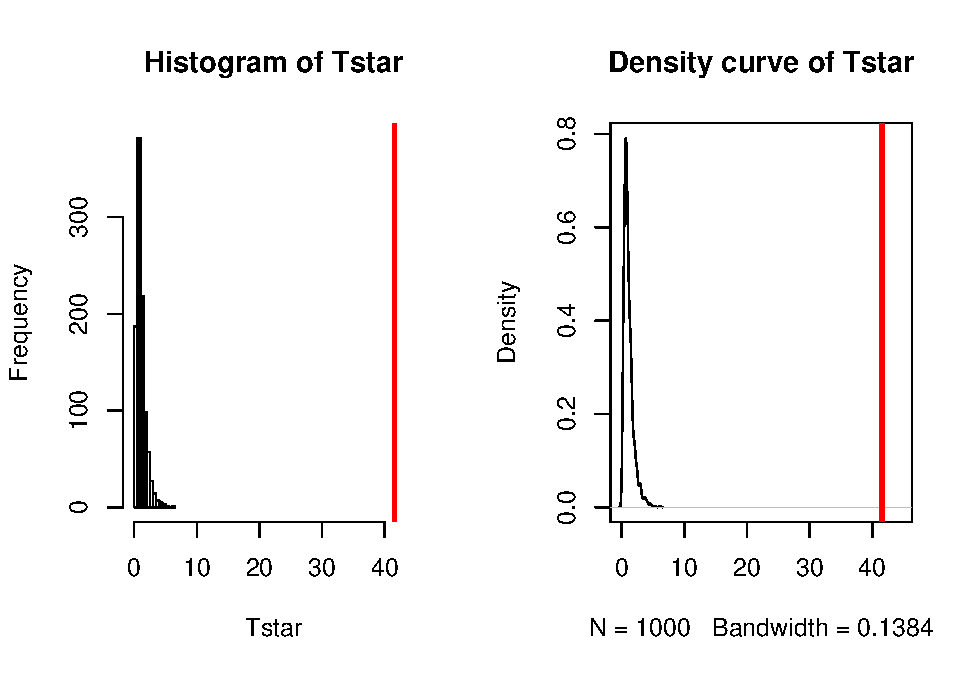
\includegraphics{03-oneWayAnova_files/figure-latex/Figure3-16-1.pdf}
  \caption{\label{fig:Figure3-16}(ref:fig3-16)}
  \end{figure}

  \begin{itemize}
  \tightlist
  \item
    \textbf{The permutation p-value was reported as 0. This should be
    reported as p-value\textless{}0.001} since we did 1000 permutations
    and found that none of the permuted \(F\)-statistics, \(F^*\), were
    larger than the observed \(F\)-statistic of 41.56. The permuted
    results do not exceed 6 as seen in Figure \ref{fig:Figure3-16}, so
    the observed result is \emph{really unusual} relative to the null
    hypothesis. As suggested previously, the parametric and
    nonparametric approaches should be similar here and they were.
  \end{itemize}
\item
  \textbf{Make a decision}:

  \begin{itemize}
  \tightlist
  \item
    Reject \(H_0\) since the p-value is less than 5\%.
  \end{itemize}
\item
  \textbf{Write a conclusion}:

  \begin{itemize}
  \item
    There is evidence at the 5\% significance level that the different
    treatments (combinations of OJ/VC and dosage levels) \textbf{cause
    some} difference in the \textbf{true} mean tooth growth for
    \textbf{these} guinea pigs.

    \begin{itemize}
    \item
      We can make the causal statement of the treatment causing
      differences because the treatments were randomly assigned but
      these inferences only apply to these guinea pigs since they were
      not randomly selected from a larger population.
    \item
      Remember that we are making inferences to the population or true
      means and not the sample means and want to make that clear in any
      conclusion. When there is not a random sample from a population it
      is more natural to discuss the true means since we can't extend to
      the population values.
    \item
      The alternative is that there is some difference in the true means
      -- be sure to make the wording clear that you aren't saying that
      all the means differ. In fact, if you look back at Figure
      \ref{fig:Figure3-14}, the means for the 2 mg dosages look almost
      the same so we will have a tough time arguing that all groups
      differ. The \(F\)-test is about finding evidence of some means.
      The next section will provide some additional tools to get more
      specific about the source of those detected differences.
    \end{itemize}
  \end{itemize}
\end{enumerate}

Before we leave this example, we should revisit our model estimates and
interpretations. The default model parameterization is into the
reference-coding. Running the model \texttt{summary} function on
\texttt{m2} provides the estimated coefficients:

\begin{Shaded}
\begin{Highlighting}[]
\KeywordTok{summary}\NormalTok{(m2)}
\end{Highlighting}
\end{Shaded}

\begin{verbatim}
## 
## Call:
## lm(formula = len ~ Treat, data = ToothGrowth)
## 
## Residuals:
##    Min     1Q Median     3Q    Max 
##  -8.20  -2.72  -0.27   2.65   8.27 
## 
## Coefficients:
##             Estimate Std. Error t value Pr(>|t|)
## (Intercept)   13.230      1.148  11.521 3.60e-16
## TreatVC.0.5   -5.250      1.624  -3.233  0.00209
## TreatOJ.1      9.470      1.624   5.831 3.18e-07
## TreatVC.1      3.540      1.624   2.180  0.03365
## TreatOJ.2     12.830      1.624   7.900 1.43e-10
## TreatVC.2     12.910      1.624   7.949 1.19e-10
## 
## Residual standard error: 3.631 on 54 degrees of freedom
## Multiple R-squared:  0.7937, Adjusted R-squared:  0.7746 
## F-statistic: 41.56 on 5 and 54 DF,  p-value: < 2.2e-16
\end{verbatim}

For some practice with the reference coding used in these models, let's
find the estimates for observations for a couple of the groups. To work
with the parameters, you need to start with diagnosing the baseline
category that was used by considering which level is not displayed in
the output. The \texttt{levels} function can list the groups in a
categorical variable and their coding in the data set. The first level
is usually the baseline category but you should check this in the model
summary as well.

\begin{Shaded}
\begin{Highlighting}[]
\KeywordTok{levels}\NormalTok{(ToothGrowth}\OperatorTok{$}\NormalTok{Treat)}
\end{Highlighting}
\end{Shaded}

\begin{verbatim}
## [1] "OJ.0.5" "VC.0.5" "OJ.1"   "VC.1"   "OJ.2"   "VC.2"
\end{verbatim}

There is a \texttt{VC.0.5} in the second row of the model summary, but
there is no row for \texttt{0J.0.5} and so this must be the baseline
category. That means that the fitted value or model estimate for the OJ
at 0.5 mg/day group is the same as the \texttt{(Intercept)} row or
\(\hat{\alpha}\), estimating a mean tooth growth of 13.23 microns when
the pigs get OJ at a 0.5 mg/day dosage level. You should always start
with working on the baseline level in a reference-coded model. To get
estimates for any other group, then you can use the \texttt{(Intercept)}
estimate and add the deviation for the group of interest. For
\texttt{VC.0.5}, the estimated mean tooth growth is
\(\hat{\alpha} + \hat{\tau}_2 = \hat{\alpha} + \hat{\tau}_{VC0.5}=13.23 + (-5.25)=7.98\)
microns. It is also potentially interesting to directly interpret the
estimated difference (or deviation) between \texttt{OJ0.5} (the
baseline) and \texttt{VC0.5} (group 2) that is
\(\hat{\tau}_{VC0.5}= -5.25\): we estimate that the mean tooth growth in
\texttt{VC0.5} is 5.25 microns shorter than it is in \texttt{OJ0.5}.
This and many other direct comparisons of groups are likely of interest
to researchers involved in studying the impacts of these supplements on
tooth growth and the next section will show us how to do that
(correctly!).

The reference-coding is still going to feel a little uncomfortable so
the comparison to the cell-means model and exploring the effect plot can
help to reinforce that both models patch together the same estimated
means for each group. For example, we can find our estimate of 7.98
microns for the VC0.5 group in the output and Figure
\ref{fig:Figure3-17}. Also note that Figure \ref{fig:Figure3-17} is the
same whether you plot the results from \texttt{m2} or \texttt{m3}.




\begin{Shaded}
\begin{Highlighting}[]
\NormalTok{m3<-}\KeywordTok{lm}\NormalTok{(len}\OperatorTok{~}\NormalTok{Treat}\OperatorTok{-}\DecValTok{1}\NormalTok{,}\DataTypeTok{data=}\NormalTok{ToothGrowth)}
\KeywordTok{summary}\NormalTok{(m3)}
\end{Highlighting}
\end{Shaded}

\begin{verbatim}
## 
## Call:
## lm(formula = len ~ Treat - 1, data = ToothGrowth)
## 
## Residuals:
##    Min     1Q Median     3Q    Max 
##  -8.20  -2.72  -0.27   2.65   8.27 
## 
## Coefficients:
##             Estimate Std. Error t value Pr(>|t|)
## TreatOJ.0.5   13.230      1.148  11.521 3.60e-16
## TreatVC.0.5    7.980      1.148   6.949 4.98e-09
## TreatOJ.1     22.700      1.148  19.767  < 2e-16
## TreatVC.1     16.770      1.148  14.604  < 2e-16
## TreatOJ.2     26.060      1.148  22.693  < 2e-16
## TreatVC.2     26.140      1.148  22.763  < 2e-16
## 
## Residual standard error: 3.631 on 54 degrees of freedom
## Multiple R-squared:  0.9712, Adjusted R-squared:  0.968 
## F-statistic:   303 on 6 and 54 DF,  p-value: < 2.2e-16
\end{verbatim}

\begin{Shaded}
\begin{Highlighting}[]
\KeywordTok{par}\NormalTok{(}\DataTypeTok{mfrow=}\KeywordTok{c}\NormalTok{(}\DecValTok{1}\NormalTok{,}\DecValTok{2}\NormalTok{))}
\KeywordTok{plot}\NormalTok{(}\KeywordTok{allEffects}\NormalTok{(m2))}
\end{Highlighting}
\end{Shaded}

\begin{figure}
\centering
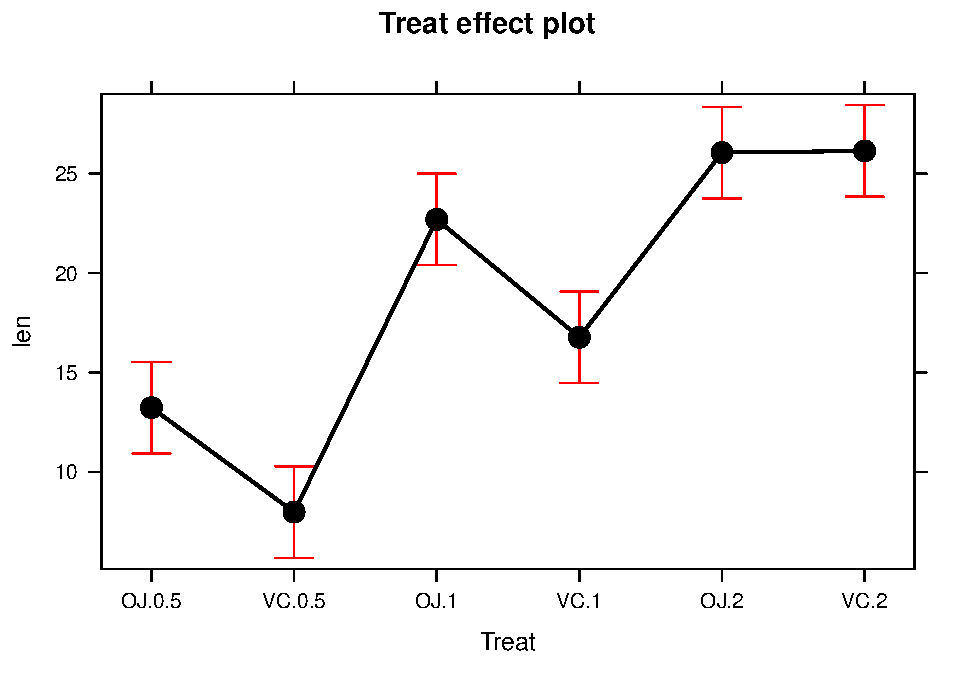
\includegraphics{03-oneWayAnova_files/figure-latex/Figure3-17-1.pdf}
\caption{\label{fig:Figure3-17}Effect plot of the One-Way ANOVA model for the toothgrowth
data.}
\end{figure}

\section{Multiple (pair-wise) comparisons using Tukey's HSD and the
compact letter display}\label{section3-6}

With evidence that the true means are likely not all equal, many
researchers want to know which groups show evidence of differing from
one another. This provides information on the source of the overall
difference that was detected and detailed information on which groups
differed from one another. Because this is a shot-gun/unfocused sort of
approach, some people think it is an over-used procedure. Others feel
that it is an important method of addressing detailed questions about
group comparisons in a valid way. For example, we might want to know if
OJ is dosage level and these methods will allow us to get an answer to
this sort of question. It also will test for differences between the
OJ,0.5 and VC,2 groups and every other pair of levels that you can
construct. This method actually takes us back to the methods in Chapter
\ref{chapter2} where we compared the means of two groups except that we
need to deal with potentially many pair-wise comparisons, making an
adjustment to account for that inflation in Type I errors that occurs
due to many tests being performed at the same time. There are many
different statistical methods to make all the pair-wise comparisons, but
we will employ the most commonly used one, called \textbf{\emph{Tukey's
Honest Significant Difference}} (Tukey's HSD) method\footnote{When this
  procedure is used with unequal group sizes it is also sometimes called
  Tukey-Kramer's method.}. The name suggests that not using it could
lead to a dishonest answer and that it will give you an honest result.
It is more that if you don't do some sort of correction for all the
tests you are performing, you might find some
\textbf{\emph{spurious}}\footnote{We often use ``spurious'' to describe
  falsely rejected null hypotheses, but there are also called false
  detections.} results. There are other methods that could be used to do
a similar correction and also provide ``honest'' inferences; we are just
going to learn one of them.

Generally, the general challenge in this situation is that if you
perform many tests at the same time, you inflate the Type I error rate.
We can define the \textbf{\emph{family-wise error rate}} as the
probability that at least one error is made on a set of tests or, more
compactly, Pr(At least 1 error is made) where Pr() is the probability of
an event occurring. The family-wise error is meant to capture the
overall situation in terms of measuring the likelihood of making a
mistake if we consider many tests, each with some chance of making their
own mistake, and focus on how often we make at least one error when we
do many tests. A quick probability calculation shows the magnitude of
the problem. If we start with a 5\% significance level test, then
Pr(Type I error on one test) =0.05 and the Pr(no errors made on one
test) =0.95, by definition. This is our standard hypothesis testing
situation. Now, suppose we have \(m\) independent tests, then

Figure \ref(fig:Figure3-18) shows how the probability of having at least
one false detection grows rapidly with the number of tests. The plot
stops at 100 tests since it is effectively a 100\% chance of at least on
false detection. It might seem like doing 100 tests is a lot, but in
Genetics research it is possible to consider situations where millions
of tests are considered so these are real issues to be concerned about
in many situations. Researchers want to make sure that when they report
a ``significant'' result that it is really likely to be a real result
and will show up as a difference in the next data set they
collect.\footnote{Many researchers are now collecting multiple data sets
  to use in a single study and using one data set to identify
  interesting results and then using a validation or test data set that
  they withheld from initial analysis to verify that the first results
  are also present in that second data set.}




\begin{figure}
\centering
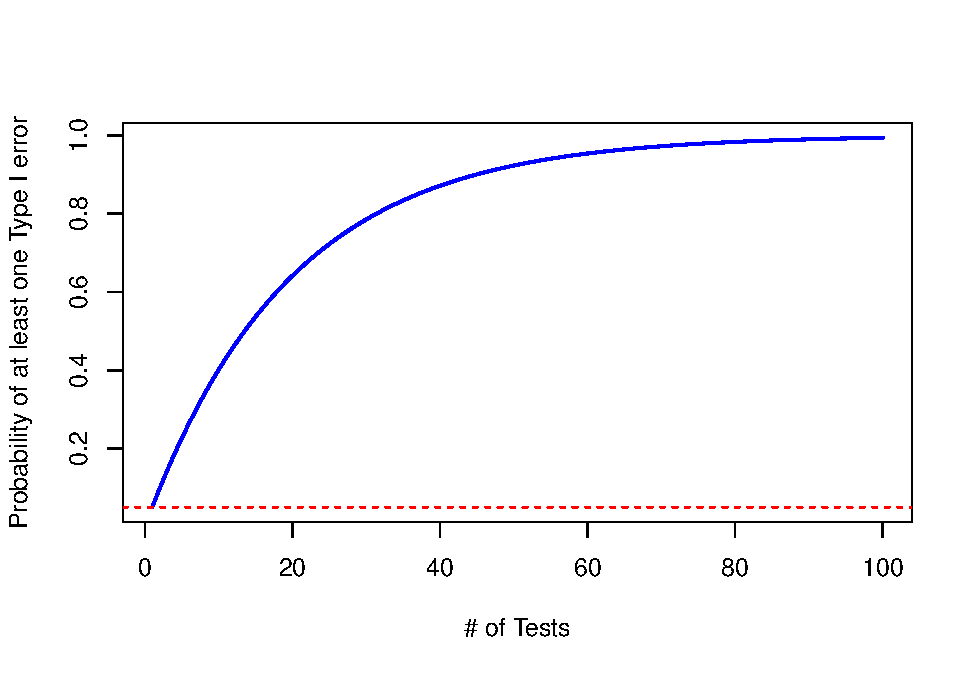
\includegraphics{03-oneWayAnova_files/figure-latex/Figure3-18-1.pdf}
\caption{\label{fig:Figure3-18}Plot of family-wise error rate as the number of tests
performed increases. Dashed line indicates 0.05.}
\end{figure}

In pair-wise comparisons between all the pairs of means in a One-Way
ANOVA, the number of tests is based on the number of pairs. We can
calculate the number of tests using \(J\) choose 2,
\(\begin{pmatrix}J\\2\end{pmatrix}\), to get the number of unique pairs
of size 2 that we can make out of \(J\) individual treatment levels. We
don't need to explore the combinatorics formula for this, as the
\texttt{choose} function can give us the answers:

\begin{Shaded}
\begin{Highlighting}[]
\KeywordTok{choose}\NormalTok{(}\DecValTok{3}\NormalTok{,}\DecValTok{2}\NormalTok{)}
\end{Highlighting}
\end{Shaded}

\begin{verbatim}
## [1] 3
\end{verbatim}

\begin{Shaded}
\begin{Highlighting}[]
\KeywordTok{choose}\NormalTok{(}\DecValTok{4}\NormalTok{,}\DecValTok{2}\NormalTok{)}
\end{Highlighting}
\end{Shaded}

\begin{verbatim}
## [1] 6
\end{verbatim}

\begin{Shaded}
\begin{Highlighting}[]
\KeywordTok{choose}\NormalTok{(}\DecValTok{5}\NormalTok{,}\DecValTok{2}\NormalTok{)}
\end{Highlighting}
\end{Shaded}

\begin{verbatim}
## [1] 10
\end{verbatim}

\begin{Shaded}
\begin{Highlighting}[]
\KeywordTok{choose}\NormalTok{(}\DecValTok{6}\NormalTok{,}\DecValTok{2}\NormalTok{)}
\end{Highlighting}
\end{Shaded}

\begin{verbatim}
## [1] 15
\end{verbatim}

So if you have three groups (prisoner rating study), there are 3 unique
pairs to compare. For six groups, like in the guinea pig study, we have
to consider 15 tests to compare all the unique pairs of groups. 15 tests
seems like enough that we should be worried about inflated family-wise
error rates. Fortunately, the Tukey's HSD method controls the
family-wise error rate at your specified level (say 0.05) across any
number of pair-wise comparisons. This means that the overall rate of at
least one Type I error is controlled at the specified significance
level, often 5\%. To do this, each test must use a slightly more
conservative cut-off than if just one test is performed and the
procedure helps us figure out how much more conservative we need to be.

Tukey's HSD starts with focusing on the difference between the groups
with the largest and smallest means (\(\bar{y}_{max}-\bar{y}_{min}\)).
If \((\bar{y}_{max}-\bar{y}_{min}) \le \text{Margin of Error}\) for the
difference in the means, then all other pairwise differences, say
\(\vert \bar{y}_j - \bar{y}_{j'}\vert\), for two groups \(j\) and
\(j'\), will be less than or equal to that margin of error. This also
means that any confidence intervals for any difference in the means will
contain 0. Tukey's HSD selects a critical value so that
(\(\bar{y}_{max}-\bar{y}_{min}\)) will be less than the margin of error
in 95\% of data sets drawn from populations with a common mean. This
implies that in 95\% of data sets in which all the population means are
the same, all confidence intervals for differences in pairs of means
will contain 0. Tukey's HSD provides confidence intervals for the
difference in true means between groups \(j\) and \(j'\),
\(\mu_j-\mu_{j'}\), for all pairs where \(j \ne j'\), using

\[(\bar{y}_j - \bar{y}_{j'}) \mp \frac{q^*}{\sqrt{2}}\sqrt{\text{MS}_E\left(\frac{1}{n_j}+
\frac{1}{n_{j'}}\right)}\]

where
\(\frac{q^*}{\sqrt{2}}\sqrt{\text{MS}_E\left(\frac{1}{n_j}+ \frac{1}{n_{j'}}\right)}\)
is the margin of error for the intervals. The distribution used to find
the multiplier, \(q^*\), for the confidence intervals is available in
the \texttt{qtukey} function and generally provides a slightly larger
multiplier than the regular \(t^*\) from our two-sample \(t\)-based
confidence interval discussed in Chapter \ref{chapter2}. We will use the
\texttt{confint}, \texttt{cld}, and \texttt{plot} functions applied to
output from the \texttt{glht} function (all from the \texttt{multcomp}
package; \citet{Hothorn2008}, \citep{R-multcomp}) to easily get the
required comparisons from our ANOVA model. Unfortunately, its code
format is a little complicated -- but there are just two places to
modify the code, by including the model name and after \texttt{mcp}
(stands for multiple comparisons) in the \texttt{linfct} option, you
need to include the explanatory variable name as
\texttt{VARIABLENAME="Tukey"}. The last part is to get the TukeyHSD
multiple comparisons run on our explanatory variable. Once we obtain the
intervals, we can use them to test
\(H_0: \mu_j = \mu_{j'} \text{ vs } HA: \mu_j \ne \mu{j'}\) by assessing
whether 0 is in the confidence interval for each pair. If 0 is in the
interval, then there is no evidence of a difference for that pair. If 0
is not in the interval, then we reject \(H_0\) and have evidence
\emph{at the specified family-wise significance level} of a difference
for that pair. You will see a switch to using the word ``detection'' to
describe rejected null hypotheses of no difference as it can help to
write up these results. The following code provides the numerical and
graphical\footnote{The plot of results usually contains all the labels
  of groups but if the labels are long or there many groups, sometimes
  the row labels are hard to see even with re-sizing the plot to make it
  taller in RStudio. The numerical output is useful as a guide to help
  you read the plot.} results of applying Tukey's HSD to the linear
model for the Guinea Pig data:





\begin{Shaded}
\begin{Highlighting}[]
\KeywordTok{par}\NormalTok{(}\DataTypeTok{mfrow=}\KeywordTok{c}\NormalTok{(}\DecValTok{1}\NormalTok{,}\DecValTok{1}\NormalTok{))}
\KeywordTok{require}\NormalTok{(multcomp)}
\NormalTok{Tm2 <-}\StringTok{ }\KeywordTok{glht}\NormalTok{(m2, }\DataTypeTok{linfct =} \KeywordTok{mcp}\NormalTok{(}\DataTypeTok{Treat =} \StringTok{"Tukey"}\NormalTok{))}
\KeywordTok{confint}\NormalTok{(Tm2)}
\end{Highlighting}
\end{Shaded}

\begin{verbatim}
## 
##   Simultaneous Confidence Intervals
## 
## Multiple Comparisons of Means: Tukey Contrasts
## 
## 
## Fit: lm(formula = len ~ Treat, data = ToothGrowth)
## 
## Quantile = 2.9545
## 95% family-wise confidence level
##  
## 
## Linear Hypotheses:
##                      Estimate lwr      upr     
## VC.0.5 - OJ.0.5 == 0  -5.2500 -10.0482  -0.4518
## OJ.1 - OJ.0.5 == 0     9.4700   4.6718  14.2682
## VC.1 - OJ.0.5 == 0     3.5400  -1.2582   8.3382
## OJ.2 - OJ.0.5 == 0    12.8300   8.0318  17.6282
## VC.2 - OJ.0.5 == 0    12.9100   8.1118  17.7082
## OJ.1 - VC.0.5 == 0    14.7200   9.9218  19.5182
## VC.1 - VC.0.5 == 0     8.7900   3.9918  13.5882
## OJ.2 - VC.0.5 == 0    18.0800  13.2818  22.8782
## VC.2 - VC.0.5 == 0    18.1600  13.3618  22.9582
## VC.1 - OJ.1 == 0      -5.9300 -10.7282  -1.1318
## OJ.2 - OJ.1 == 0       3.3600  -1.4382   8.1582
## VC.2 - OJ.1 == 0       3.4400  -1.3582   8.2382
## OJ.2 - VC.1 == 0       9.2900   4.4918  14.0882
## VC.2 - VC.1 == 0       9.3700   4.5718  14.1682
## VC.2 - OJ.2 == 0       0.0800  -4.7182   4.8782
\end{verbatim}

\begin{Shaded}
\begin{Highlighting}[]
\NormalTok{old.par <-}\StringTok{ }\KeywordTok{par}\NormalTok{(}\DataTypeTok{mai=}\KeywordTok{c}\NormalTok{(}\FloatTok{1.5}\NormalTok{,}\DecValTok{2}\NormalTok{,}\DecValTok{1}\NormalTok{,}\DecValTok{1}\NormalTok{)) }\CommentTok{#Makes room on the plot for the group names}
\KeywordTok{plot}\NormalTok{(Tm2)}
\end{Highlighting}
\end{Shaded}

\begin{figure}
\centering
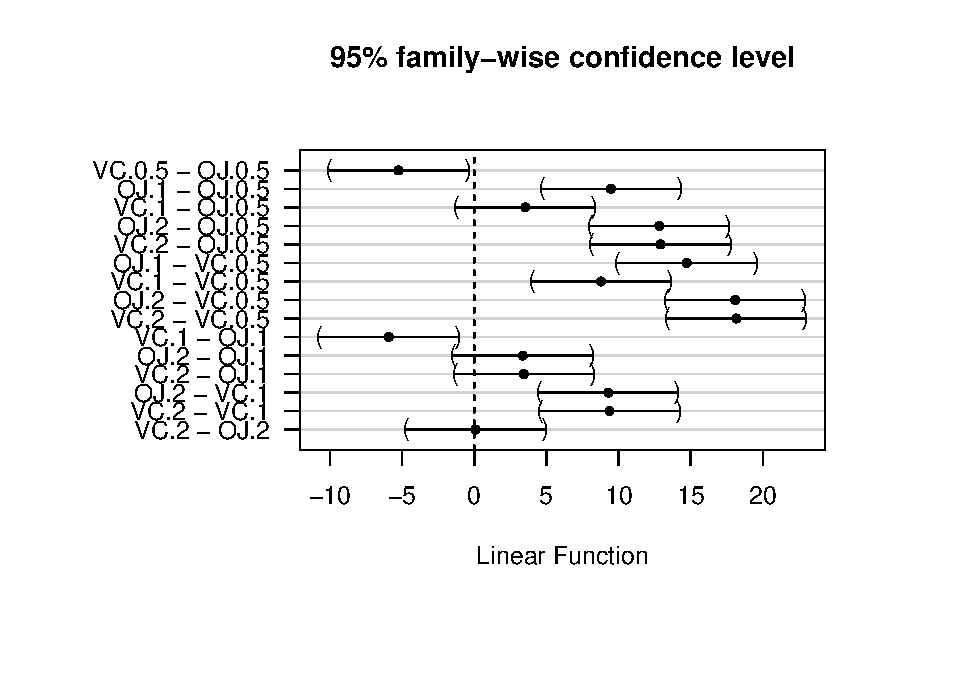
\includegraphics{03-oneWayAnova_files/figure-latex/Figure3-19-1.pdf}
\caption{\label{fig:Figure3-19}Graphical display of pair-wise comparisons from Tukey's
HSD for the Guinea Pig data. Any confidence intervals that do not
contain 0 provide evidence of a difference in the groups.}
\end{figure}

Figure \ref{fig:Figure3-19} contains confidence intervals for the
difference in the means for all 15 pairs of groups. For example, the
first row in the plot contains the confidence interval OJ.0.5). In the
numerical output, you can find that this 95\% family-wise confidence
interval goes from -10.05 to -0.45 microns (\texttt{lwr} and
\texttt{upr} in the numerical output provide the CI endpoints). This
interval does not contain 0 since its upper end point is -0.45 microns
and so we can now say that there is evidence that OJ and VC have
different true mean growth rates at the 0.5 mg dosage level. We can go
further and say that we are 95\% confident that the difference in the
true mean tooth growth between VC.0.5 and OJ.0.5 (VC.0.5-OJ.0.5) is
between -10.05 and -0.45 microns, after adjusting for comparing all the
pairs of groups. But there are fourteen more similar intervals\ldots{}

If you put all these pair-wise tests together, you can generate an
overall interpretation of Tukey's HSD results that discusses sets of
groups that are not detectably different from one another and those
groups that were distinguished from other sets of groups. To do this,
start with listing out the groups that do are not detectably different
(CIs contain 0), which, here, only occurs for four of the pairs. The CIs
that contain 0 are for the pairs VC.1 and OJ.0.5, OJ.2 and OJ.1, VC.2
and OJ.1, and, finally, VC.2 and OJ.2. So VC.2, OJ.1, and OJ.2 are all
not detectably different from each other and VC.1 and OJ.0.5 are also
not detectably different. If you look carefully, VC.0.5 is detected as
different from every other group. So there are basically three sets of
groups that can be grouped together as ``similar'': VC.2, OJ.1, and
OJ.2; VC.1 and OJ.0.5; and VC.0.5. Sometimes groups overlap with some
levels not being detectably different from other levels that belong to
different groups and the story is not as clear as it is in this case. An
example of this sort of overlap is seen in the next section.

There is a method that many researchers use to more efficiently generate
and report these sorts of results that is called a \textbf{\emph{compact
letter display}} (CLD, \citet{Piepho2004}). The \texttt{cld} function
can be applied to the results from \texttt{glht} to generate the CLD
that we can use to provide a ``simple'' summary of the sets of groups.
In this discussion, we define a \textbf{set as a union of different
groups that can contain one or more members} and the member of these
groups are the different treatment levels.

\begin{Shaded}
\begin{Highlighting}[]
\KeywordTok{cld}\NormalTok{(Tm2)}
\end{Highlighting}
\end{Shaded}

\begin{verbatim}
## OJ.0.5 VC.0.5   OJ.1   VC.1   OJ.2   VC.2 
##    "b"    "a"    "c"    "b"    "c"    "c"
\end{verbatim}

Groups with the same letter are not detectably different (are in the
same set) and groups that are detectably different get different letters
(are in different sets). Groups can have more than one letter to reflect
``overlap'' between the sets of groups and sometimes a set of groups
contains only a single treatment level (VC.0.5 is a set of size 1). Note
that if the groups have the same letter, this does not mean they are the
same, just that there is \textbf{no evidence of a difference for that
pair}. If we consider the previous output for the CLD, the ``a'' set
contains VC.0.5, the ``b'' set contains OJ.1, OJ.2, and VC.2, and the
``c'' set contains OJ.0.5 and VC.1. These are exactly the groups of
treatment levels that we obtained by going through all fifteen pairwise
results.

One benefit of this work is that the CLD letters can be added to a
beanplot to help fully report the results and understand the sorts of
differences Tukey's HSD detected.




\begin{figure}
\centering
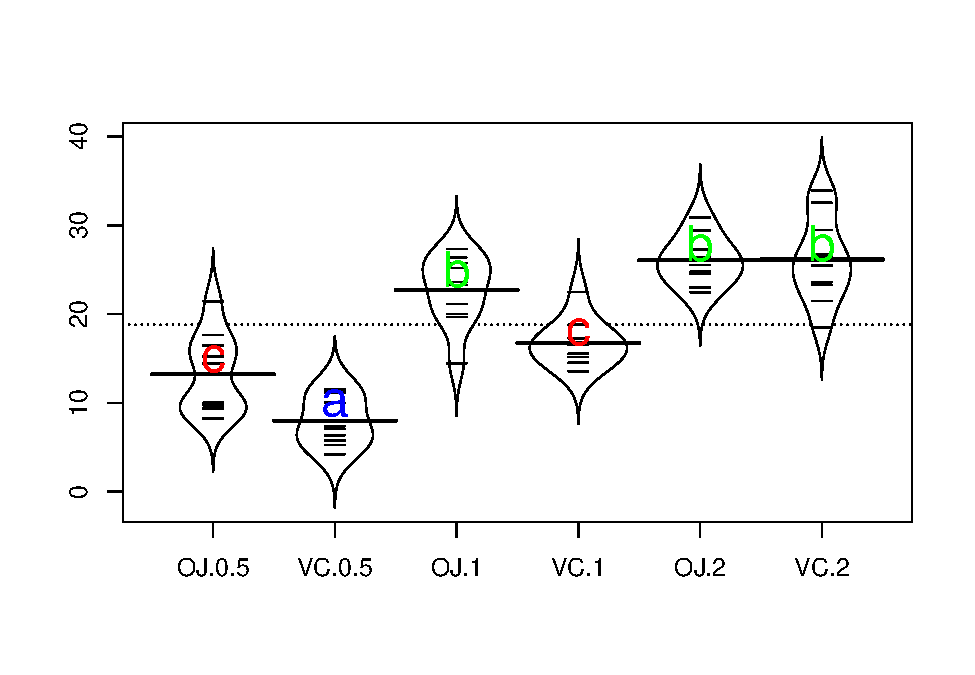
\includegraphics{03-oneWayAnova_files/figure-latex/Figure3-20-1.pdf}
\caption{\label{fig:Figure3-20}Beanplot of tooth growth by group with Tukey?s HSD compact
letter display.}
\end{figure}

The lines with text in them are involved in placing text on the figure
but are something you could do in image editing software just as easily.
Figure \ref{fig:Figure3-20} enhances the discussion by showing that the
``\textcolor{blue}{\textbf{a}}'' group with VC.0.5 had the lowest
average tooth growth, the ``\textcolor{red}{\textbf{c}}'' group had
intermediate tooth growth for treatments OJ.0.5 and VC.1, and the
highest growth rates came from OJ.1, OJ.2, and VC.2. Even though VC.2
had the highest average growth rate, we are not able to prove that its
true mean is any higher than the other groups labeled with
``\textcolor{green}{\textbf{b}}''. Hopefully the ease of getting to the
story of the Tukey's HSD results from a plot like this explains why it
is common to report results using these methods instead of reporting 15
confidence intervals.

There are just a couple of other details to mention on this set of
methods. First, note that we interpret the set of confidence intervals
simultaneously: We are 95\% confident that \textbf{ALL} the intervals
contain the respective differences in the true means (this is a
\textbf{\emph{family-wise interpretation}}). These intervals are
adjusted from our regular 2 sample \(t\) intervals from Chapter
\ref{chapter2} to allow this stronger interpretation. Specifically, they
are wider. Second, if sample sizes are unequal in the groups, Tukey's
HSD is conservative and provides a family-wise error rate that is lower
than the nominal (or specified) level. In other words, it fails less
often than expected and the intervals provided are a little wider than
needed, containing all the pairwise differences at higher than the
nominal confidence level of (typically) 95\%. Third, this is a
parametric approach and violations of normality and constant variance
will push the method in the other direction, potentially making the
technique dangerously liberal. Nonparametric approaches to this problem
are also possible, but will not be considered here.

\section{Pair-wise comparisons for Prisoner Rating
data}\label{section3-7}

In our previous work with the prisoner rating data, the overall ANOVA
test provided only marginal evidence of some difference in the true
means across the three groups with a p-value=0.067. Tukey's HSD does not
require you to find a small from your overall \(F\)-test to employ the
methods but if you apply it to situations with p-values larger than your
\emph{a priori} significance level, you are unlikely to find any pairs
that are detected as being different. Some statisticians suggest that
you shouldn't employ follow-up tests such as Tukey's HSD when there is
not sufficient evidence to reject the overall null hypothesis and would
be able to reasonably criticize the following results. But for the sake
of completeness, we can find the pair-wise comparison results at our
typical 95\% family-wise confidence level in this situation, with the
three confidence intervals displayed in Figure \ref{fig:Figure3-21}.




\begin{Shaded}
\begin{Highlighting}[]
\NormalTok{lm2<-}\KeywordTok{lm}\NormalTok{(Years}\OperatorTok{~}\NormalTok{Attr, }\DataTypeTok{data=}\NormalTok{MockJury)}
\KeywordTok{require}\NormalTok{(multcomp)}
\NormalTok{Tm2 <-}\StringTok{ }\KeywordTok{glht}\NormalTok{(lm2, }\DataTypeTok{linfct =} \KeywordTok{mcp}\NormalTok{(}\DataTypeTok{Attr =} \StringTok{"Tukey"}\NormalTok{))}
\KeywordTok{confint}\NormalTok{(Tm2)}
\end{Highlighting}
\end{Shaded}

\begin{verbatim}
## 
##   Simultaneous Confidence Intervals
## 
## Multiple Comparisons of Means: Tukey Contrasts
## 
## 
## Fit: lm(formula = Years ~ Attr, data = MockJury)
## 
## Quantile = 2.3751
## 95% family-wise confidence level
##  
## 
## Linear Hypotheses:
##                               Estimate lwr     upr    
## Average - Beautiful == 0      -0.3596  -2.2969  1.5776
## Unattractive - Beautiful == 0  1.4775  -0.4730  3.4280
## Unattractive - Average == 0    1.8371  -0.1258  3.8001
\end{verbatim}

\begin{Shaded}
\begin{Highlighting}[]
\KeywordTok{cld}\NormalTok{(Tm2)}
\end{Highlighting}
\end{Shaded}

\begin{verbatim}
##    Beautiful      Average Unattractive 
##          "a"          "a"          "a"
\end{verbatim}

\begin{Shaded}
\begin{Highlighting}[]
\NormalTok{old.par <-}\StringTok{ }\KeywordTok{par}\NormalTok{(}\DataTypeTok{mai=}\KeywordTok{c}\NormalTok{(}\FloatTok{1.5}\NormalTok{,}\FloatTok{2.5}\NormalTok{,}\DecValTok{1}\NormalTok{,}\DecValTok{1}\NormalTok{)) }\CommentTok{#Makes room on the plot for the group names}
\KeywordTok{plot}\NormalTok{(Tm2)}
\end{Highlighting}
\end{Shaded}

\begin{figure}
\centering
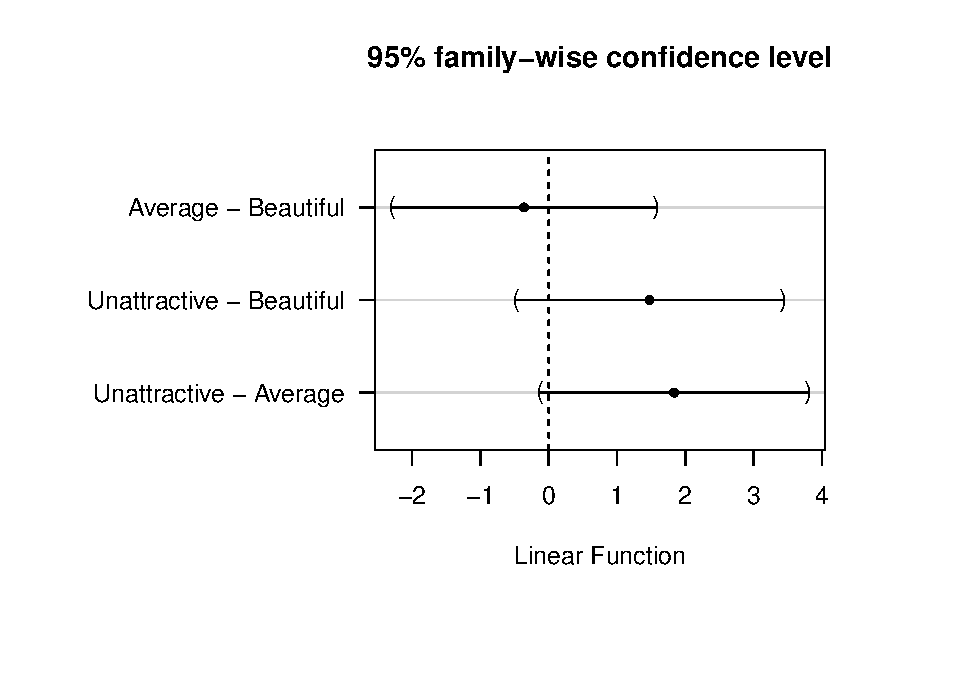
\includegraphics{03-oneWayAnova_files/figure-latex/Figure3-21-1.pdf}
\caption{\label{fig:Figure3-21}Tukey's HSD confidence interval results at the 95\%
family-wise confidence level.}
\end{figure}

At the family-wise 5\% significance level, there are no pairs that are
detectably different -- they all get the same letter of ``a''. Now we
will produce results for the reader that thought a 10\% significance was
suitable for this application before seeing any of the results. We just
need to change the confidence level or significance level that the CIs
or tests are produced with inside the functions. For the
\texttt{confint} function, the \texttt{level} option is the confidence
level and for the \texttt{cld}, it is the family-wise significance
level. Note that 90\% confidence corresponds to a 10\% significance
level.



\begin{Shaded}
\begin{Highlighting}[]
\KeywordTok{confint}\NormalTok{(Tm2,}\DataTypeTok{level=}\FloatTok{0.9}\NormalTok{)}
\end{Highlighting}
\end{Shaded}

\begin{verbatim}
## 
##   Simultaneous Confidence Intervals
## 
## Multiple Comparisons of Means: Tukey Contrasts
## 
## 
## Fit: lm(formula = Years ~ Attr, data = MockJury)
## 
## Quantile = 2.0739
## 90% family-wise confidence level
##  
## 
## Linear Hypotheses:
##                               Estimate lwr     upr    
## Average - Beautiful == 0      -0.3596  -2.0513  1.3320
## Unattractive - Beautiful == 0  1.4775  -0.2257  3.1806
## Unattractive - Average == 0    1.8371   0.1231  3.5512
\end{verbatim}

\begin{Shaded}
\begin{Highlighting}[]
\KeywordTok{cld}\NormalTok{(Tm2,}\DataTypeTok{level=}\FloatTok{0.1}\NormalTok{)}
\end{Highlighting}
\end{Shaded}

\begin{verbatim}
##    Beautiful      Average Unattractive 
##         "ab"          "a"          "b"
\end{verbatim}

\begin{Shaded}
\begin{Highlighting}[]
\NormalTok{old.par <-}\StringTok{ }\KeywordTok{par}\NormalTok{(}\DataTypeTok{mai=}\KeywordTok{c}\NormalTok{(}\FloatTok{1.5}\NormalTok{,}\FloatTok{2.5}\NormalTok{,}\DecValTok{1}\NormalTok{,}\DecValTok{1}\NormalTok{)) }\CommentTok{#Makes room on the plot for the group names}
\KeywordTok{plot}\NormalTok{(}\KeywordTok{confint}\NormalTok{(Tm2,}\DataTypeTok{level=}\NormalTok{.}\DecValTok{9}\NormalTok{))}
\end{Highlighting}
\end{Shaded}

\begin{figure}
\centering
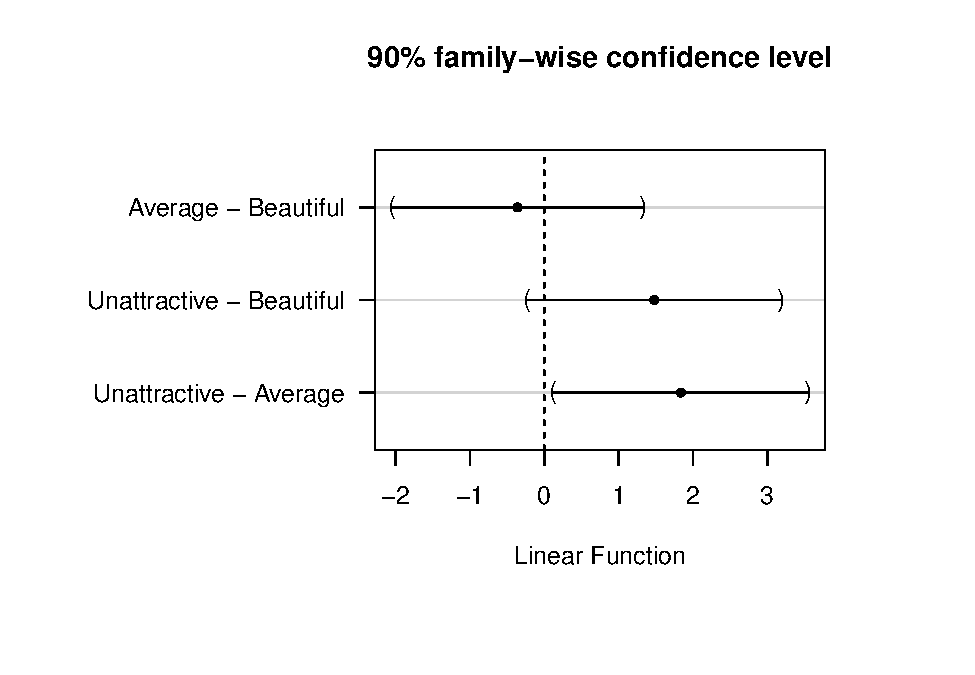
\includegraphics{03-oneWayAnova_files/figure-latex/Figure3-22-1.pdf}
\caption{\label{fig:Figure3-22}Tukey's HSD 90\% family-wise confidence intervals.}
\end{figure}

With family-wise 10\% significance and 90\% confidence levels, the
\emph{Unattractive} and \emph{Average} picture groups are detected as
being different but the \emph{Average} group is not detected as
different from \emph{Beautiful} and \emph{Beautiful} is not detected to
be different from \emph{Unattractive}. This leaves the ``overlap'' of
groups across the sets of groups that was noted earlier. The
\emph{Beautiful} level is not detected as being dissimilar from levels
in two different sets and so gets two different letters.

The beanplot (Figure \ref{fig:Figure3-23}) helps to clarify some of the
reasons for this set of results. The detection of a difference between
\emph{Average} and \emph{Unattractive} just barely occurs and the mean
for \emph{Beautiful} is between the other two so it ends up not being
detectably different from either one. This sort of overlap is actually a
fairly common occurrence in these sorts of situations so be prepared a
mixed set of letters for some levels.







\begin{Shaded}
\begin{Highlighting}[]
\KeywordTok{beanplot}\NormalTok{(Years}\OperatorTok{~}\NormalTok{Attr,}\DataTypeTok{data=}\NormalTok{MockJury,}\DataTypeTok{log=}\StringTok{""}\NormalTok{,}\DataTypeTok{col=}\StringTok{"white"}\NormalTok{,}\DataTypeTok{method=}\StringTok{"jitter"}\NormalTok{)}
\KeywordTok{text}\NormalTok{(}\KeywordTok{c}\NormalTok{(}\DecValTok{1}\NormalTok{),}\KeywordTok{c}\NormalTok{(}\DecValTok{5}\NormalTok{),}\StringTok{"ab"}\NormalTok{,}\DataTypeTok{col=}\StringTok{"blue"}\NormalTok{,}\DataTypeTok{cex=}\DecValTok{2}\NormalTok{)}
\KeywordTok{text}\NormalTok{(}\KeywordTok{c}\NormalTok{(}\DecValTok{2}\NormalTok{),}\KeywordTok{c}\NormalTok{(}\FloatTok{4.8}\NormalTok{),}\StringTok{"a"}\NormalTok{,}\DataTypeTok{col=}\StringTok{"green"}\NormalTok{,}\DataTypeTok{cex=}\DecValTok{2}\NormalTok{)}
\KeywordTok{text}\NormalTok{(}\KeywordTok{c}\NormalTok{(}\DecValTok{3}\NormalTok{),}\KeywordTok{c}\NormalTok{(}\FloatTok{6.5}\NormalTok{),}\StringTok{"b"}\NormalTok{,}\DataTypeTok{col=}\StringTok{"red"}\NormalTok{,}\DataTypeTok{cex=}\DecValTok{2}\NormalTok{)}
\end{Highlighting}
\end{Shaded}

\begin{figure}
\centering
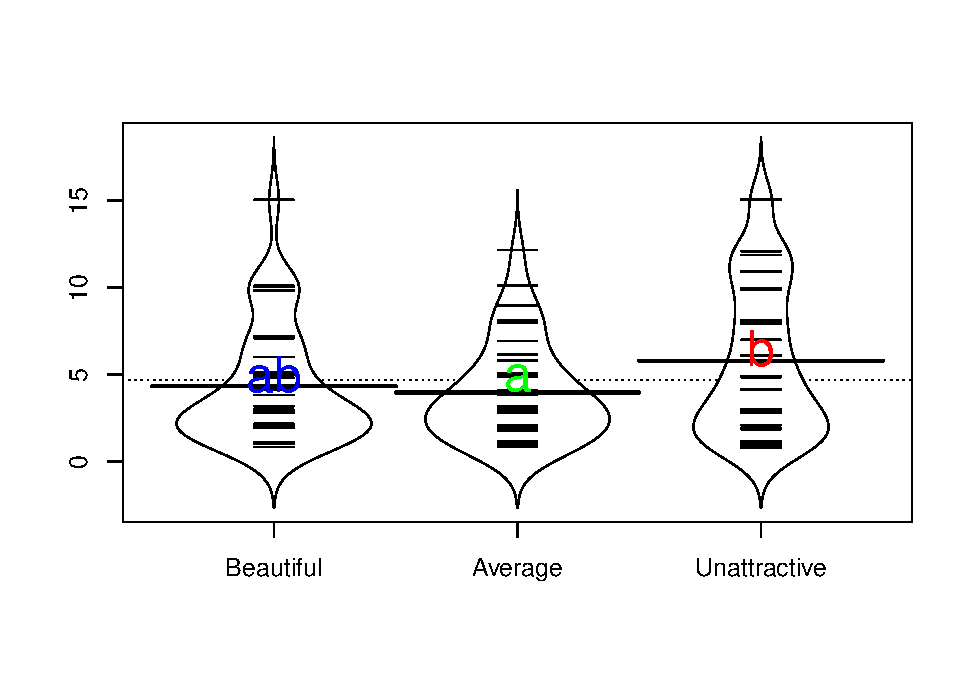
\includegraphics{03-oneWayAnova_files/figure-latex/Figure3-23-1.pdf}
\caption{\label{fig:Figure3-23}Beanplot of sentences with compact letter display results
from 10\% family-wise significance level Tukey's HSD. \emph{Average} and
\emph{Unattractive} picture groups are detected as being different and
are displayed as belonging to different groups. \emph{Beautiful} picture
responses are not detected as different from the other two groups.}
\end{figure}

\section{Chapter Summary}\label{section3-8}

In this chapter, we explored methods for comparing a quantitative
response across \(J\) groups (\(J \ge 2\)), with what is called the
One-Way ANOVA procedure. The initial test is based on assessing evidence
against a null hypothesis of no groups. There are two different methods
for estimating these One-Way ANOVA models: the cell-means model and the
reference-coded versions of the model. There are times when either model
will be preferred, but for the rest of the text, the reference coding is
used (sorry!). The ANOVA \(F\)-statistic, often presented with
underlying information in the ANOVA table, provides a method of
assessing evidence against the null hypothesis either using permutations
or via the \(F\)-distribution. Pair-wise comparisons using Tukey's HSD
provide a method for comparing all the groups and are a nice complement
to the overall ANOVA results. A compact letter display was shown that
enhanced the interpretation of Tukey's HSD result.

In the guinea pig example, we are left with some lingering questions
based on these results. It appears that the effect of \emph{dosage}
changes as a function of the \emph{delivery method} (OJ, VC) because the
size of the differences between OJ and VC change for different dosages.
These methods can't directly assess the question of whether the effect
of delivery method is the same or not across the different dosages. In
chapter \ref{chapter4}, the two variables, \emph{Dosage} and
\emph{Delivery method} are modeled as two separate variables so we can
consider their effects both separately and together. This allows more
refined hypotheses, such as \emph{Is the effect of delivery method the
same for all dosages?}, to be tested. This will introduce new models and
methods for analyzing data where there are two factors as explanatory
variables in a model for a quantitative response variable in what is
called the Two-Way ANOVA.

\section{Summary of important R code}\label{section3-9}

The main components of R code used in this chapter follow with
components to modify in red, remembering that any R packages mentioned
need to be installed and loaded for this code to have a chance of
working:

\begin{itemize}
\item
  \textcolor{red}{MODELNAME} \textless{}-
  lm(\textcolor{red}{Y}\textasciitilde{}\textcolor{red}{X},
  data=\textcolor{red}{DATASETNAME})

  \begin{itemize}
  \item
    Probably the most frequently used command in R.
  \item
    Here it is used to fit the reference-coded One-Way ANOVA model with
    Y as the response variable and X as the grouping variable, storing
    the estimated model object in MODELNAME.
  \end{itemize}
\item
  \textcolor{red}{MODELNAME} \textless{}-
  lm(\textcolor{red}{Y}\textasciitilde{}\textcolor{red}{X}-1,
  data=\textcolor{red}{DATASETNAME})

  \begin{itemize}
  \tightlist
  \item
    Fits the cell means version of the One-Way ANOVA model.
  \end{itemize}
\item
  summary(\textcolor{red}{MODELNAME})

  \begin{itemize}
  \tightlist
  \item
    Generates model summary information including the estimated model
    coefficients, SEs, t-tests, and p-values.
  \end{itemize}
\item
  anova(\textcolor{red}{MODELNAME})

  \begin{itemize}
  \item
    Generatesthe ANOVA table but \textbf{must only be run on the
    reference-coded version of the model}.
  \item
    Results are incorrect if run on the cell-means model since the
    reduced model under the null is that the mean of all the
    observations is 0!
  \end{itemize}
\item
  pf(\textcolor{red}{FSTATISTIC},df1=\textcolor{red}{NUMDF},df2=\textcolor{red}{DENOMDF},
  lower.tail=F)

  \begin{itemize}
  \tightlist
  \item
    Finds the p-value for an observed \(F\)-statistic with NUMDF and
    DENOMDF degrees of freedom.
  \end{itemize}
\item
  par(mfrow=c(2,2)); plot(\textcolor{red}{MODELNAME})

  \begin{itemize}
  \tightlist
  \item
    Generates four diagnostic plots including the Residuals vs Fitted
    and Normal Q-Q plot.
  \end{itemize}
\item
  plot(allEffects(\textcolor{red}{MODELNAME}))

  \begin{itemize}
  \item
    Requires the \texttt{effects} package be loaded.
  \item
    Plots the estimated model component.
  \end{itemize}
\item
  Tm2 \textless{}- glht(\textcolor{red}{MODELNAME},
  linfct=mcp(\textcolor{red}{X}=``Tukey'')); confint(Tm2); plot(Tm2);
  cld(Tm2)

  \begin{itemize}
  \item
    Requires the \texttt{multcomp} package to be installed and loaded.
  \item
    Can only be run on the reference-coded version of the model.
  \item
    Generates the text output and plot for Tukey's HSD as well as the
    compact letter display.
  \end{itemize}
\end{itemize}

\section{Practice problems}\label{section3-10}

For these practice problems, you will work with the cholesterol data set
from the \texttt{multcomp} package that was used to generate the Tukey's
HSD results. To load the data set and learn more about the study, use
the following code:

\begin{verbatim}
require(multcomp)
data(cholesterol)
help(cholesterol)
\end{verbatim}

3.1. Graphically explore the differences in the changes in Cholesterol
levels for the five levels using boxplots and beanplots.

3.2. Is the design balanced?

3.3. Complete all 6+ steps of the hypothesis test using the parametric
\(F\)-test, reporting the ANOVA table and the distribution of the test
statistic under the null.

3.4. Discuss the scope of inference using the information that the
treatment levels were randomly assigned to volunteers in the study.

3.5. Generate the permutation distribution and find the p-value. Compare
the parametric p-value to the permutation test results.

3.6. Perform Tukey's HSD on the data set. Discuss the results -- which
pairs were detected as different and which were not? Bigger reductions
in cholesterol are good, so are there any levels you would recommend or
that might provide similar reductions?

3.7. Find and interpret the CLD and compare that to your interpretation
of results from 3.6.

\chapter{Two-Way ANOVA}\label{chapter4}

\chapter{Chi-square tests}\label{chapter5}

\chapter{Correlation and Simple Linear Regression}\label{chapter6}

\chapter{Simple linear regression inference}\label{chapter7}

\chapter{Multiple linear regression}\label{chapter8}

\chapter{Case studies}\label{chapter9}

\chapter{Placeholder}\label{placeholder-2}

\bibliography{packages,references}


\end{document}
